% Inicio do texto da tese
% Por: Habib S. D. Montoya
% Doutorado em Fisica
% Orientador: Martín Makler
% CBPF - Centro Brasileiro de Pesquisas Fisicas
% Atualizado:26/10/2007
\documentclass[a4paper,12pt,twoside]{report}
\linespread{1.5}
% putting the package to be used
\usepackage[pdftex]{color,graphicx}
\usepackage{mathrsfs}
\usepackage{fancyhdr}
\usepackage[x11names]{xcolor}
\usepackage{float}
\usepackage{wrapfig}
\usepackage{ccaption}
\usepackage{amssymb}
\usepackage{amsmath}
\usepackage{dcolumn}
\usepackage{subfigure}%{ccaption}
\usepackage{longtable}
\usepackage[thinspace,amssymb]{SIunits}
\usepackage{subeqnarray}
% defining new commands
\newcommand{\HRule}{\rule{\linewidth}{0.5mm}}
% \newcommand{\sen}[×][×]{×}
%adding SI units.
\addunit{\parsec}{pc}
\addunit{\asec}{\arcsecond}
\addunit{\am}{\arcminute}
% \addunit{\ergios}{ergs}
% \addunit{\anho}{yr}
% \addunit{\edad}{\giga\anho}
% defining some abbreviations

%%%%%%%%%%%%%%%%%%% Mandeep's Definitions %%%%%%%%%%%%%%%%%%%%%%%%%%%%

\def\prtl{\partial}
\def \scriptf {\mathcal{F}}
\def \scriptg {\mathcal{G}}
\def\vecrz{\vec{r}_{0}}
\def\hatr{\hat{r}}
\def\hatth{\hat{\theta}}
\def\dfdt{{d \overline{f}_0(\theta) \over d \theta}}
\def\fbar{\overline{f}_1}
\def\wrt{with respect to}

\def\yone{y_{01}}
\def\ytwo{y_{02}}

\def\eqref{eq.~(\ref}
\def\secref{Sec.~\ref}
\def\figref{Fig.~\ref}

\def\vecy{\vec{y}}

\def\cost{\cos \theta}
\def\sint{\sin \theta}

\def\costwot{\cos 2 \theta}
\def\sintwot{\sin 2 \theta}

\def\ppr{{\partial \over \partial r }}
\def\ppt{{\partial \over \partial \theta }}

\def\oor{{1 \over r}}
\def\oorsq{{1 \over r^2}}
\def\twoor{{2 \over r}}

\def\pprsq{{\partial^2 \over \partial r^2 }}
\def\pptsq{{\partial^2 \over \partial \theta^2 }}
\def\pprt{{\partial^2 \over \partial r \partial \theta }}



\def\pptsqfz{{\partial^2 f_0 \over \partial \theta^2 }}
\def\pptfone{{\partial f_1 \over \partial \theta }}
\def\pptfz{{\partial f_0 \over \partial \theta }}


\def\oorsq{{1 \over r^2}}

\def\lp{\left(}
\def\rp{\right)}

\def\lbracket{\left[}
\def\rbracket{\right]}

\def\half{{1 \over 2}}

%%%%%%%%%%%%%%%%%%%%% Habib's Definitions %%%%%%%%%%%%%%%%%%%%%%%%%%%%%%%%
\def \eps {\epsilon}
\def \al {\alpha}
\def \re {R_{\mathrm{E}}}
\def \rre{\dfrac{r}{\re}}
\def \prre {\left( \rre\right)}
\def \te {\theta}
\def \tep {\theta_p}
\def \kt {\kappa_2}
\def \kex {\kappa_{_{\mathrm{EX}}}}
\def \gex {\gamma_{_{\mathrm{EX}}}}
\def \xie {\zeta_{_{\mathrm{E}}}}
\def \xer {\xi_{_{\mathrm{E}}}}
\def \ae {a_{1\eta}}
\def \be {a_{2\eta}}


%%%%%%%%%%%%%%%%%%%%% Gabriel's Definitions %%%%%%%%%%%%%%%%%%%%%%%%%%%%%%%%




%%%%%%%%%%%%%%%%%%%%% Another Definitions %%%%%%%%%%%%%%%%%%%%%%%%%%%%%%%%%%%%
\def \beq {\begin{equation}}
\def \eeq {\end{equation}}
\def \beqn {\begin{equation*}}
\def \eeqn {\end{equation*}}
\def\bea{\begin{eqnarray}}
\def\eea{\end{eqnarray}}

% reference to journal (see Astronomy and Astrophysics)
\def \etal {\emph{et al.}}
\def \aap {A\&A}
\def \mnras {MNRAS}
\def \apj  {ApJ}
%% Definiendo as cores a usar
% \DefineNamedColor{algo}{hnamei}{hmodel-listi}{hspec-listi}
%
%_____________________________Formata??o da p\'agina_____________________________________%
% \usepackage{layout}
% % Vertical
% \setlength{\voffset}{-2.50 cm}
% \setlength{\topmargin}{0.6 cm}
% \setlength{\headheight}{0.5 cm}
% \setlength{\headsep}{1.5 cm}
% \setlength{\topskip}{0.3in}
% \setlength{\textheight}{25 cm}
% % Horizontal
% \setlength{\hoffset}{0.0cm}
% \setlength{\evensidemargin}{0.4 cm}
% \setlength{\oddsidemargin}{0.4 cm}
% \setlength{\textwidth}{16 cm}
% \setlength{\marginparsep}{0.25 cm}
% \setlength{\marginparwidth}{2.54 cm}
\usepackage[margin=2.cm,asymmetric]{geometry}
\bibliographystyle{unsrt}
%_________________________________________________________________________________%

\begin{document}
%_______________________Paginas Iniciais_______________________________________________%
\pagenumbering{roman}\setcounter{page}{2}\pagestyle{plain}
\begin{titlepage}

\begin{center}


% Upper part of the page
% 
\includegraphics[totalheight=2.5cm,width=0.15\textwidth]{graficos/misc/Logo_CBPF-2.jpg}\\[1cm]

\textbf{\Large Preliminary Report  }\\[3.5cm]

% Title
\HRule \\[0.6cm]
{ \large \bfseries Perturbative Approach in Strong Gravitational Lensing}\\[0.4cm]

\HRule \\[1.0cm]

\vspace{2.0cm}

{\Large \textbf{\textit{Gabriel Caminha, Habib D\'umet-Montoya, Mandeep S.~S.~Gill, Mart\'in Makler}}}\\
{\large \textbf{DES-Brazil / DES Strong Lensing Working Group}}\\[1.5cm]

\vfill

% Bottom of the page
{\large Rio de Janeiro, Julho de 2011}

\end{center}

\begin{flushright}
    
\includegraphics[scale=0.5]{graphics/SLSG-Logo.jpg}
\end{flushright}

\end{titlepage} 
%\include{abstract}
\tableofcontents
\listoffigures %\addcontentsline{toc}{section}{List of Figures}
% \listoftables  %\addcontentsline{toc}{section}{Lista de Tabelas}


%________________________Corpo de Texto________________________________________________%
%
% Now set up the main body of the paper:
\newpage\pagenumbering{arabic}\setcounter{page}{1}%\pagestyle{plain}
\setlength{\headheight}{30pt}
\pagestyle{fancy}
\renewcommand{\chaptermark}[1]{\markboth{#1}{}}
\renewcommand{\sectionmark}[1]{\markright{#1}{}}
%
\fancyhf{}
\fancyhead[LE,RO]{\thepage}
\fancyhead[RE]{\textbf{\textit{\nouppercase{\leftmark}}}}
\fancyhead[LO]{\textit{\nouppercase{\rightmark}}}
%
\fancypagestyle{plain}{ %
\fancyhf{} % remove everything
\renewcommand{\headrulewidth}{0.4pt} % remove lines as well
\renewcommand{\footrulewidth}{0.4pt}}
%
\chapter{Introduction}

\section{Remarks on Notation}

{\bf Source Plane Coordinates}
\begin{itemize}
\item{ $ y = (y_1, y_2) $ are Cartesian coordinates of a point in the source plane}
\item{   $r_s $ is the radial coordinate of a point in the source plane}
\item{   $r_0 $ is the radial coordinate to the center of a circular source in the source plane}

\item{   $\vec{r}_0 =(\yone,\ytwo)$ is the vector to the center of a circular source in the source plane}

\item{ $R_0 $ is the vector distance from the center of circular
  source to its edge in the source plane}

\item{ $\eta_s$ is the ellipticity of an object in the source plane}

\end{itemize}

{\bf Lens Plane Coordinates}

\begin{itemize}
\item{ $ x = (x_1, x_2) $ are Cartesian coordinates of a point in the lens plane}
\item{ $  (r, \theta) $ are polar coordinates of a point in the lens plane}
\item{ $\re$ is Einstein Radius of the critical curve in the lens plane}
\end{itemize}



\section{Summary of primary equations}

From \secref{sec:BasicIdeas}, we have the division of the potential into
axisymmetric and non-axisymmetric pieces:

eq.~(\ref{eq:potsplit}): $\phi  =  \phi_0 + \eps \psi$.

Which we expand into

\eqref{eq:tse2}): $\phi  = \sum_{n=0}^\infty \left[ C_n + \eps f_n  \right] (r-\re)^n$

with definitions

\eqref{eq:Cndef}): $C_n \equiv {1 \over n!} \left. {d^n \phi_0 \over dr^n }\right|_{\re}$

\eqref{eq:fndef}): $f_n(\theta) \equiv  {1 \over n!} \left. {d^n \psi(\theta) \over dr^n }\right|_{\re}$

And this leads to the equation for the mapping of the lens to source plane in terms of the $f_{0,1}$ functions:

\eqref{eq:rsexpanded}):  $y = \left[ \kt x - f_1 \right] \hat{r} - {1 \over \re} {\prtl f_0 \over \prtl \te}  \hat{\theta}$

with  $\kt \equiv 1-2 C_2$
\\
\\
\\
{\bf Lens Curves}
Now we move to the ``lens curves'' -- the equations for the critical curves and caustics.

First, for the tangential critical curves:

\eqref{eq:critcurves}): $x=\frac{1}{\kt}\left[f_1+\frac{1}{\re}\frac{d^2f_0}{d\te^2}\right] \label{xte}$

And for the caustics:

\eqref{eq:xcaustic}): $y_{1_\mathrm{caust}} = \frac{1}{\re}\frac{d^2f_0}{d\te^2}\cos{\te}+\frac{1}{\re}\frac{df_0}{d\te}\sin{\te}$

\eqref{eq:ycaustic}): $y_{2_\mathrm{caust}} = \frac{1}{\re}\frac{d^2f_0}{d\te^2}\sin{\te}-\frac{1}{\re}\frac{df_0}{d\te}\cos{\te}$
\\
\\
\\
{\bf Arcs}

For a circular extended source, the radial arc position in the lens plane is

\eqref{eq:xsoln}):  $x = \frac{1}{\kappa_2}\left[ \overline{f}_{1}(\theta) \pm \sqrt{R_0^2 - \left( \frac{1}{\re}\frac{\partial \overline{f}_0(\theta)}{\partial \theta} \right)^2} \right] $

With $\overline{f}_i(\theta) \equiv f_i(\theta) + (x_0 \cos \te + y_0 \sin \te)\re^{1-i}, \;\; i=0,1 $

And
\eqref{eq:parametricarcs}): $\vec{r}= \left[(\re +x)\cos{\te},(\re+x)\sin{\te}\right], \quad 0 \leq \te < 2\pi$

are the Cartesian coordinates for this in parametric form.
\\
\\
For an elliptical extended source where the source is oriented at an angle $\theta_0$ \wrt\ the semi-major axis of the central potential, the radial arc position in the lens plane is

\eqref{eq:ellipsource}): $x = \frac{1}{\kappa_2} \left\{\bar{f}_{1}(\theta) +%
\frac{\eta_s\sin(2\tilde{\theta})}{S}\left(\frac{1}{\re}\dfrac{\partial%
\bar{f}_0(\theta)}{\partial \theta}\right) \pm \frac{1}{S}\sqrt{SR_{0}^2 -%
(1-\eta_s^2)\left[ \frac{1}{\re}\frac{\partial \bar{f}_0(\theta)}{\partial
\theta}\right]^2}  \right\}$

with $ S \equiv 1-\eta_s\cos{(2\tilde{\te})}$, and $\tilde{\te} = \theta - \theta_0$

And again
\eqref{eq:parametricarcs}): $\vec{r}= \left[(\re +x)\cos{\te},(\re+x)\sin{\te}\right], \quad 0 \leq \te < 2\pi$

are the Cartesian coordinates for this in parametric form.


{\bf }



\chapter{Perturbative Approach in Strong Lensing}
\section{\label{sec:BasicIdeas} Basic Ideas}


Let us assume that the two-dimensional projected density $\Sigma$ of a
strong gravitational lens system is axially symmetric and centered at
the origin. Let us assume that the lens is dense enough and that the
distances among the observer, lens, and soruce are such that the
critical density is reached within a radius $\re$. Under such an
hypothesis, the image of a point source placed in the source plane at
the origin will be a perfect ring at $\re$. However, if the source is
not perfectly at the center, or the potential is not perfectly
axisymmetric, the perfect ring is broken into arcs.

To investigate this fact, we will use the lens equation $\vec{r}_s =
\vec{r} - \vec{\alpha}$, where $\vec{r}_s$ is the angular position of
the point source in the source plane (see fig. 5 in \cite{NarayanAndB}
for this configuration), $\vec{r} = r \hat{r} $ is the angular
position of the point source in the image plane, and $\vec{\alpha}$ is
the deflection angle, which is equal to the gradient of the 2D
projected lens potential $\phi$ in the image plane, which in polar coordinates
is

\beq
\vec{\alpha} = \nabla_r \phi = \dfrac{\prtl  \phi}{\prtl r} \hat{r} +
\dfrac{1}{r} \dfrac{\prtl  \phi}{\prtl \theta} \hat{\theta}.
\eeq

(also, we use $ \hat{r}, \hat{\theta}$ in place of Alard's $\hat{u}_r,
\hat{u}_\theta$).

Thus
\bea
\vec{r}_s & = & r \hat{r} - \left( \dfrac{\prtl  \phi}{\prtl r} \hat{r} + {1
\over r} \dfrac{\prtl  \phi }{ \prtl \theta} \hat{\theta} \right) \label{eq:rs}
\\
& = & \left( r -  \dfrac{\prtl \phi}{\prtl r} \right) \hat{r} -  \dfrac{1}{r}
\dfrac{\prtl \phi }{\prtl \theta} \hat{\theta}
\eea

Now let us go to the simplest case of an on-axis point source with
perfectly axially symmetric potential $\phi(\vec{r}) = \phi_0(|\vec{r}|)$.  In
this case
$r_s = 0$ and  ${\prtl \phi_0 \over \prtl \theta} = 0$ since there is no
angular variation of the potential.

Thus, eq.(\ref{eq:rs}) reduces to

\beq
0 =  r -  {\prtl  \phi \over \prtl r}
\eeq

the solution to which is the Einstein Radius

\beq
\label{eq:einsteinradius}
  \re =  \left. {\prtl  \phi \over \prtl r} \right|_{\re} 
\eeq

where the derivative of the potential is to be evaluated at the Einstein radius,
$ \re$.

This indicates the point source is spread into a circle of radius $ \re $ in the
image plane.

We now take the first step of perturbing the situation:

\bea
\label{eq:rspert}
\vec{r}_s & = & \eps \vec{y}, \\
\phi( \vec{r} ) & = & \phi_0(|\vec{r}|) + \eps \psi( \vec{r} )
\label{eq:potsplit},
\eea

which imply we have moved the source off-axis, and added a non-axially
symmetric potential, both to the exact same order $\eps$ by
assumption.  Note that the perturbed distance $y$ is in the source plane.

Note that this changes the notation of the first eq in Alard eq.~3
(which doesn't make much sense, of course).

We now write the image position also as a perturbation around the
Einstein Radius, using eq.(\ref{eq:rspert}) to modify
eq.(\ref{eq:einsteinradius}) into

\beq
\label{eq:rpert}
r = \re +  \eps x
\eeq

which changes the notation in Alard eq.~4 (which is somewhat weird notation,
since his $dr$ is not necessarily a small distance), and we do not follow
his convention of setting $\re \equiv 1$.

Note that now the perturbed distance $x$ is in the image plane.

To recap: $r_s, y$ are in the source plane, while $r, x$ are in the image plane.

Now we do a Taylor series expansion of the potential about the Einstein ring
radius:

\beq
\phi = \phi_0 + \eps \psi = \sum_{n=0}^\infty {1 \over n!} \left. {d^n \phi_0
\over dr^n }\right|_{\re} (r-\re)^n + \eps {1 \over n!} \left. {d^n \psi \over
dr^n }\right|_{\re} (r-\re)^n
\eeq

or

\beq
\label{eq:tse}
\phi  = \sum_{n=0}^\infty \left[ {1 \over n!} \left. {d^n \phi_0 \over dr^n
}\right|_{\re} + \eps {1 \over n!} \left. {d^n \psi \over dr^n }\right|_{\re}
\right] (r-\re)^n
\eeq

And now define

\beq
\label{eq:Cndef}
C_n \equiv {1 \over n!} \left. {d^n \phi_0 \over dr^n }\right|_{\re}
\eeq

\beq
\label{eq:fndef}
f_n(\theta) \equiv  {1 \over n!} \left. {d^n \psi \over dr^n }\right|_{\re}
\eeq

So that we can write  eq.(\ref{eq:tse}) as

\beq
\label{eq:tse2}
\phi  = \sum_{n=0}^\infty \left[ C_n + \eps f_n(\theta)  \right] (r-\re)^n
\eeq

where $f_n(\theta)$ is a one-dimensional function independent of $r$.


Now we go back and substitute \eqref{eq:rspert}) and \eqref{eq:rpert}) into
\eqref{eq:rs}) to find
\beq
\eps y = \left( \re + \eps x -  {\prtl  \phi \over \prtl r} \right) \hat{r} - {1
\over \re + \eps x}  {\prtl  \phi \over \prtl \theta} \hat{\theta}
\eeq

Now substitute \eqref{eq:tse2}) into this to find

\bea
\eps \vec{y} = \left( \re + \eps x -  {\prtl \over \prtl r} \left(
\sum_{n=0}^\infty \left[ C_n + \eps f_n  \right] (r-\re)^n  \right) \right)
\hat{r} - \\
{1 \over \re + \eps x}  {\prtl  \over \prtl \theta} \left( \sum_{n=0}^\infty
\left[ C_n + \eps f_n  \right] (r-\re)^n  \right)  \hat{\theta} \nonumber
\eea

Remembering that $C_n$ and  $f_n$ are independent of $r$, and using
\eqref{eq:rpert}), $r-\re = \eps x$ we find

\bea
\label{eq:tse3}
\eps y = \left( \re + \eps x -   \sum_{n=0}^\infty \left[ C_n + \eps f_n 
\right] n (\eps x)^{n-1}  \right) \hat{r} - \\
{1 \over \re + \eps x}  {\prtl  \over \prtl \theta} \left( \sum_{n=0}^\infty
\left[ C_n + \eps f_n  \right] (\eps x)^n  \right)  \hat{\theta} \nonumber
\eea

Let us expand \eqref{eq:tse3} in orders, first the zero'th order piece in
$\eps$:

\beq
0 =  \left(\re - C_1 \right) \hat{r} \rightarrow \re = C_1 = \left. \prtl \phi
\over \prtl \theta \right|_{\re},
\eeq

so that we reassuringly recover the Einstein ring solution.

Next the first order piece in $\eps$:

\beq
\eps \vec{y} = \left( \eps x - (2 C_2 \eps x + \eps f_1 ) \right) \hat{r} - {1
\over \re} \eps {\prtl f_0 \over \prtl \theta } \hat{\theta}
\eeq

where the coefficient of $C_2$ was expanded to order $n=2$, that of
the $f_1$ term to order $n=1$, and that of the $\prtl f_1 \over \prtl
\theta$ term ro order $n=0$.  

%Bit involved, but this is how to get each term proportional to $\eps$.

%Now we will return to the ``physical variables'' $\eps \vec{y} = \vec{r}_s,
%\eps x = \Delta r

Now divide through by $\eps$ and collect terms:

\beq
 \vecy = \left[ (1-2 C_2) x -  f_1 \right] \hat{r} - {1 \over \re} {\prtl f_0
\over \prtl \te} \hat{\theta}
\eeq

or, defining $\kt = 1-2 C_2$

\beq
\label{eq:rsexpanded}
\vecy = ( \kt x - f_1 ) \hat{r} - {1 \over \re} {\prtl f_0 \over \prtl \te} 
\hat{\theta}
\eeq

which is Alard eq.8 (remember he set $\re \equiv 1$).


\section{Conditions for the Validity of the Approximation}
%%%%%%%%%%%%%%%%%%%%%%%%%%%%%%% Habib

At first order in $\eps$ we may define

\begin{equation}
 q \equiv \frac{r}{\re}[1-\eps\,g(\te)].
\end{equation}

As the functional $\phi_0(q)$ represents the general expression
for the perturbed potential, with $q$ defined above, we may expand $\phi_0(q)$

\begin{displaymath}
 \phi_0(q)=\phi_0\left(\rre-\eps\rre\,g(\te)\right)
\end{displaymath}

\noindent in a Taylor Series around $\eps=0$, in the following way

\def\dpdq{ \left. \left( \frac{d\phi_0}{dq}\right) \right|_{\eps=0} }
\def\dpde{ \left. \left( \frac{d\phi_0}{d\eps}\right) \right|_{\eps=0} }

\begin{eqnarray}
 \phi_0(q) &\approx& \phi_0\prre+\eps \dpde \\
	  & = & \phi\prre+\eps \dpdq  \left(\frac{\prtl q}{\prtl \eps}\right)\\
	  &\approx& \phi\prre-\rre\phi_0^\prime\prre g(\te)\eps \label{key1}
\end{eqnarray}

Where we have defined $\phi_0^\prime\prre \equiv  \dpdq$.  Note, that we have
$\phi_0(q)=\phi_0\prre$ when $\eps=0$ and similarly with its derivatives.
Therefore,
taking the partial derivatives of Eq.~(\ref{key1}), it is straightforward to
verify

\begin{eqnarray}
 \re\frac{\prtl \phi}{\prtl r}&=& \phi_0^\prime\prre -%
  \eps\left[g(\te)\phi_0^\prime\prre+\rre g(\te)\phi_0^{\prime
\prime}\prre\right]\\
\frac{\re}{r}\frac{\prtl \phi}{\prtl \te}&=&-\phi_0^\prime\prre
\frac{dg(\te)}{d\te}\eps
\end{eqnarray}

(Alard eq.19).

%%%%%%%%%%%%%%%%%%%%%%%%%%%%%%%%%%%%%%%%%%%%%%%%%%%%%%%%%%%%%%%%%%%%%%%%%%%% 
\section{Critical Curves, Caustic Lines and Deformation Cross-Section in the
Perturbative Approach}

[{\bf Include an introduction discussing the importance of source-independent
``observables''}]

\subsection{The Jacobian Matrix of the transformation}

In order to obtain the equations for the critical curves, caustics and the area
of the deformation cross-section, we'll need to make coordinate transformations
between the two planes, {\it bearing in mind that there may also be coordinate
transformations involved in the process}.

More specifically, suppose that we're using the perturbed Lens Equation to pass
from the lens plane to the source plane, both in Cartesian coordinates. This
transformation is given by the Jacobian Matrix $J_{L_C\rightarrow S_C}$.
However, in the perturbative approach, a lot of the quantities are more
conveniently written in terms of polar coordinates. In the next sections, we'll
make use of the following three facts:
\bea
J_{L_C\rightarrow S_C}&=&J_{L_P\rightarrow
S_C}J_{L_C\rightarrow L_P}\label{jacobian_comp}\\
\det(AB)&=&\det A\det B\label{determinant_mult}\\
\mbox{tr}\,(AB)&=&A_{11}B_{11}+A_{12}B_{21}+A_{21}B_{12}+A_{22}B_{22}\,,\mbox{
for $2\times 2$ matrices}\label{trace}
\eea
We also recall that the components of $J_{L_C\rightarrow L_P}$ are given by:
\begin{eqnarray}
\frac{\prtl r}{\prtl x_1}&=&\cos{\te}\label{drdx1}   \\
\frac{\prtl \te}{\prtl x_1}&=&-\frac{\sin{\te}}{r}\label{dtedx1}\\
\frac{\prtl r}{\prtl x_2}&=&\sin{\te}\label{drdx2}\\
\frac{\prtl \te}{\prtl x_2}&=&\frac{\cos{\te}}{r}\label{dte2dx2}
\end{eqnarray}

\subsection{Critical Curves and Caustics}

We will now obtain the equations for the critical curves in the lens
plane, which correspond to the caustic curves in the source plane.

First write \eqref{eq:rsexpanded}) in Cartesian coordinates (writing
the unit polar vectors as \eqref{eq:unitvs}), and taking
$\vec{y}=(y_1,y_2)$ in the source plane and $\vec{r}=(r,\te)$ in the
lens plane:
%Note that as we have not considered the position of the source,
%we have $\bar{f}_i=f_i$ and therefore
\begin{eqnarray}
y_{1} &=& (\kt x - f_1)\cos{\te}+\frac{1}{\re}\frac{d f_0}{d\te}\sin{\te}
\label{y_1}\\
y_{2} &=& (\kt x - f_1)\sin{\te}-\frac{1}{\re}\frac{d f_0}{d\te}\sin{\te}
\label{y_2},
\end{eqnarray}

It is important to stress that even though $y_{1}$ and $y_{2}$ are written in
terms of $r$ and $\te$, equations (\ref{y_1}) and (\ref{y_2}) describe the
transformation $J_{L_C\rightarrow S_C}$. Let us decompose it following eq.
(\ref{jacobian_comp}). The components of the Jacobian matrix $J_{L_P\rightarrow
S_C}$ are given by %polar to Cartesian coordinates

%\begin{equation}
%J=\frac{\prtl y_1}{\prtl r}\frac{\prtl y_2}{\prtl \te}-\frac{\prtl y_1}{\prtl
%\te}\frac{\prtl y_2}{\prtl r}.
%\label{jacob}
%\end{equation}

%The critical lines are defined by the condition $J=0$. 
\begin{eqnarray}
\frac{\prtl y_1}{\prtl r}&=& \kt \cos{\te}\label{dy1dx}   \\
\frac{\prtl y_2}{\prtl r}&=& \kt \sin{\te}\\
\frac{\prtl y_1}{\prtl \te}&=& \scriptf(\te)\sin{\te}+\scriptg(\te)\cos{\te}\\
\frac{\prtl y_2}{\prtl \te}&=&
-\scriptf(\te)\cos{\te}+\scriptg(\te)\sin{\te}\label{dy2dte}
\end{eqnarray}

using \eqref{eq:rsexpanded}), ${\prtl \over \prtl r} ={ 1 \over \epsilon}
{\prtl \over \prtl x}$ (from \eqref{eq:rpert}) and defining the functions
$\scriptf$ and $\scriptg$ as

\bea
% \begin{equation}
\scriptf(\te)&=&\frac{1}{\re}\frac{d^2f_0}{d\te^2}-(\kt x -f_1) \quad \\
% \textrm{and} \quad % \\
\scriptg(\te)&=&\frac{1}{\re}\frac{df_0}{d\te}-\frac{df_1}{d\te}
\eea
% \end{equation}

It is straightforward to verify that the determinant of this matrix is given by
$\det \left(J_{L_P\rightarrow S_C}\right)=-\kt\scriptf(\te)$. Knowing that the
Jacobian matrix $J_{L_C\rightarrow L_P}$ is the usual Jacobian transformation
from Cartesian to polar coordinates, with $\det \left(J_{L_C\rightarrow
L_P}\right)=\frac{1}{r}$, we can use eq. (\ref{determinant_mult}) to show that
\beq
J\equiv\det \left(J_{L_C\rightarrow
S_C}\right)=-\frac{\kt\scriptf(\te)}{r}\,.\label{jacobian}
\eeq

Therefore on the critical curves, where $J = 0$, we have

\begin{equation}
\label{eq:critcurves}
\Delta x_{crit}=\frac{1}{\kt}\left[f_1+\frac{1}{\re}\frac{d^2f_0}{d\te^2}\right]
\end{equation}

This is Alard eq.~30. From this last equation, the tangential critical
curve can be expressed in Cartesian coordinates in parametric form as 
\beq
\vec{r}_{\mathrm{crit}}= \left[(\re  +\Delta x_{crit})\cos{\te},(\re+\Delta x_{crit})\sin{\te}\right],\quad
0 \leq \te < 2\pi.  
\eeq

Now, substituting this last equation into eqs.~(\ref{y_1}) and
(\ref{y_2}) we obtain, the parametric equation for the tangential
caustic, i.e.,

\begin{eqnarray}
\label{eq:xcaustic}
y_{1_\mathrm{caust}} &=&
\frac{1}{\re}\frac{d^2f_0}{d\te^2}\cos{\te}+\frac{1}{\re}\frac{df_0}{d\te}\sin{
\te}\\
\label{eq:ycaustic}
y_{2_\mathrm{caust}} &=&
\frac{1}{\re}\frac{d^2f_0}{d\te^2}\sin{\te}-\frac{1}{\re}\frac{df_0}{d\te}\cos{
\te}
\end{eqnarray}

Which reduce to Alard's eqs.~31 for $\re=0$.

%%%%%%%%%%%%%%%%%%%%%%%%%%%%%%%%%  From before

Getting Alard eq.33 from the above is straight, and from there we may obtain
% I (MSSG) got most of the way to 
Alard eq.34 from 33 and 32.
% with some small hiccups..
\subsection{Eigenvalues of the Jacobian Matrix and Deformation Cross-Section}

To obtain the deformation cross-section, we want to obtain a
non-parametric expression $r_\pm (\te)$ for the limiting curves of this area. To
begin with, we recall that the eigenvalues of a $2\times 2$ non-singular matrix
$M$
are given by
\beq
\lambda_\pm=\frac{1}{2}\left(\mbox{tr}\, M\pm\sqrt{(\mbox{tr}\,M)^2-4\det
M}\right)\label{eigenvalues}
\eeq 
where $\mbox{tr}\, M$ is the trace of the matrix $M$. Using eqs. \ref{jacobian}
and \ref{trace}, it is possible to show that the eigenvalues of $J_{L_C\rightarrow
S_C}$ are given by
\bea
\lambda_{+}&=&\kt\label{eigenvalue1}\\
\lambda_{-}&=&-\frac{\scriptf(\te)}{r}=-\frac{\scriptf(\te)}{\re+x}\label{eigenvalue2}
\eea


%Therefore
%\beq
%\frac{\lambda_+}{\lambda_-}=\frac{1+\tau\sqrt{1-\alpha}}{1-\tau\sqrt{1-\alpha}}
%\label{eigenvalues_division}
%\eeq
%with $\tau=\mbox{sgn}\, M$ and $\alpha=4\frac{\det M}{(\mbox{tr}\,M)^2}$. 
If we set $\left|\frac{\lambda_+}{\lambda_-}\right|=N$ (a condition that will be used to define the
cross-section), then we can solve for the radius of the frontiers of the deformation cross-section area. The solutions are
\bea
r_{+}(\te)&=&\left|\vec{r}_{\mathrm{crit}}\right|\left(1+\frac{1}{|N|-1}\right)\label{rmax}\\
r_{-}(\te)&=&\left|\vec{r}_{\mathrm{crit}}\right|\left(1-\frac{1}{|N|+1}\right)\label{rmin}
\eea
%\beq
%\frac{\det M}{(\mbox{tr}\,M)^2}=\frac{N}{(N+1)^2}
%\eeq

\subsection{Deriving Deformation Cross-Section from Magnification and Shear Values}

Eigenvalues of the Jacobian Matrix are given by:

\bea
\mu_r &=& {1 \over 1-\kappa-\gamma} \\
\mu_t &=& {1 \over 1-\kappa+\gamma}
\eea

Now we know in Cartesian coordinates:

\bea
\kappa &=& {1 \over 2} (\Psi_{11} + \Psi_{22}) \\
\gamma_1 &=&   {1 \over 2} (\Psi_{11} - \Psi_{22}) \\
\gamma_2 &=&   \Psi_{12}  \\
\eea

with $\gamma = \sqrt{\gamma_1^2 + \gamma_2^2}$

We need to convert these Cartesian derivatives to polar ones, using:

\bea
{\partial \over \partial x } &=& \cost \ppr - \sint \oor \ppt \\
{\partial \over \partial y } &=& \sint \ppr + \cost \oor \ppt
\eea

Which lead to the expressions

\bea
{\partial^2 \over \partial x^2 } + {\partial^2 \over \partial y^2 } &=&  \pprsq +  \oorsq \pptsq + \oor \ppr \\
{\partial^2 \over \partial x^2 } - {\partial^2 \over \partial y^2 } &=&  \costwot \lp \pprsq -  \oorsq \pptsq - \oor \ppr \rp + \sintwot \lp \oorsq \ppt - \twoor \pprt \rp \\
{\partial^2 \over \partial x \partial y }  &=&  \half \sintwot \lp \pprsq -  \oorsq \pptsq - \oor \ppr \rp + \costwot \lp - \oorsq \ppt - \oor \pprt \rp
\eea

Where the first is the standard Laplacian in polar coordinates.

Using now $f_0 = \Psi$, $f_1 = {\prtl \Psi \over \prtl r}$, $f_2 = \half {\prtl^2 \Psi \over \prtl r^2}$, we obtain the following:

\bea
\kappa &=& {1 \over 2} \lp 2 f_2 + \oorsq \pptsqfz + \oor f_1 \rp \\
\gamma_1 &=&   {1 \over 2} \lp \costwot \lp 2 f_2 - \oorsq \pptsqfz - \oor f_1 \rp + \sintwot \lp \oorsq \pptfz - \twoor \pptfone \rp \rp \\
\gamma_2 &=&   \half \sintwot \lp 2 f_2 - \oorsq \pptsqfz - \oor f_1 \rp + \costwot \lp - \oorsq \pptfz - \oor \pptfone \rp  \\
\eea

%So that 

%\beq
%\gamma &=&   \sqrt \lbracket {1 \over 4}  \lp 2 f_2 - \oorsq \pptsqfz - \oor f_1 \rp^2 + \lp \oorsq \pptfz - \twoor \pptfone \rp \rp \rbracket\\
%\eeq

\section{Reconstruction of Images}

One advantage of the perturbative approach is that it allows us to
construct an analytic solution for the lensed images of sources
located near the tangential caustic.  In this section we study the
mapping of circular and elliptical contours using this formalism.

\subsection{Circular Sources}

\begin{wrapfigure}{r}{0.4\textwidth}
  \begin{center}
%  \centering{\epsfig{Fig_subsstructure.eps,width=0.45\textwidth}}
   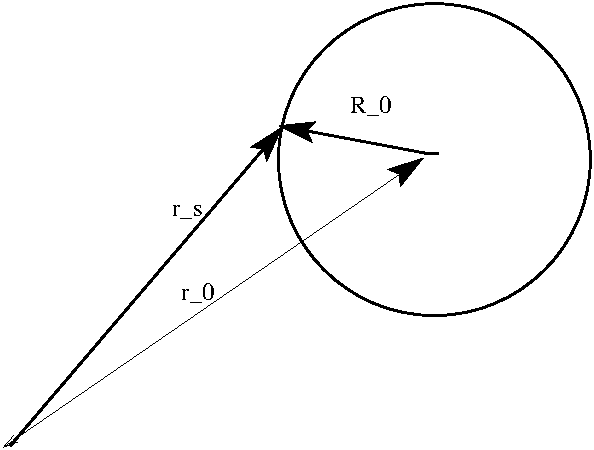
\includegraphics[width=0.35\textwidth]{graphics/sourceplane.pdf}
  \end{center}
    \caption{\label{fig:circular_source}Circular source geometry in the source
plane.}
\end{wrapfigure}

Notation: $ \vec{r}_{0}$ points from the origin (i.e center of the
source plane, which is the point we see looking directly on-axis from
us through the lens to the source) to the center of the actual source
object (which might be e.g a small face-on spiral galaxy), $
\vec{R}_{0}$ is the vectorial radius of this source from its center,
and $ \vec{r}_{s}$ is the vector from the origin to some point on the
edge of the circular source. See Fig.~\ref{fig:circular_source} for this
configuration.



Thus we have

\bea
\vec{r}_s &=&  \vec{r}_{0} + \vec{R}_{0} \\
  \vec{R}_{0} &=& \vec{r}_s - \vec{r}_{0}. \nonumber
\eea


Replacing $r_s$ by eq.~\eqref{eq:rsexpanded}, we obtain:

\beq
\label{eq:Rzero}
\vec{R_{0}} = \left[ \kappa_2 x - f_{1}(\theta) \right]\hat{r} - \frac{1}{\re}
\frac{\partial f_0(\theta)}{\partial \theta} \hat{\theta} - \vec{r_{0}}. \;\;\;
\eeq


Note that $\vec{r}_{0} = (\yone,\ytwo)$ lies in the source plane, but we
can write it in terms of the polar unit vectors

\bea
\label{eq:unitvs}
\hat{r}=(\cos\te, \sin \te) \\
\hat{\theta}=(-\sin \te, \cos \te)
\eea

 as following

\beq
\vecrz = (\vecrz \cdot \hatth) \hatth + (\vecrz \cdot \hatr) \hatr
\eeq

or


\beq
\label{eq:rzero}
\vec{r}_{0} = \left[ \yone \,  \cos \te + \ytwo \,  \sin \te \right] \hat{r} +
\left[ -\yone \,  \sin \te + \ytwo \,  \cos \te \right] \hat{\theta}.  \;\;\;
\eeq

So that eq.~\eqref{eq:Rzero} becomes

\beq
\vec{R_{0}} = \left[ \kappa_2 x - f_{1}(\theta) \right]\hat{r} - \frac{1}{\re}
\frac{\partial f_0(\theta)}{\partial \theta} \hat{\theta} -  \left[ \yone \, 
\cos \te + \ytwo \,  \sin \te \right] \hat{r} - \left[ -\yone \,  \sin \te +
\ytwo \,  \cos \te \right] \hat{\theta} \;\;\;
\eeq


Defining

\beq
\overline{f}_i(\theta) \equiv f_i(\theta) + (\yone \cos \te + \ytwo \sin
\te)\re^{1-i}, \;\; i=0,1
\eeq

this becomes

\beq
\vec{R}_{0} = \left[ \kappa_2 x - \overline{f}_{1}(\theta) \right]\hat{r} -
\frac{1}{\re} \frac{\partial \overline{f}_0(\theta)}{\partial \theta}
\hat{\theta}. \;\;\; \label{eq:Alard11}
\eeq

(Alard eq.11).

Now, taking the square of this we obtain

\beq
R_{0}^2 = \left[ \kappa_2 x - \overline{f}_{1}(\theta) \right]^2 +
\left[\frac{1}{\re} \frac{\partial \overline{f}_0(\theta)}{\partial
\theta}\right]^2. \;\;\;
\eeq

Solving this for $x(\te)$, the radius of the arc in the image plane as
a function of theta, the following two solutions are obtained:

\beq
\label{eq:xsoln}
x = \frac{1}{\kappa_2}\left[ \overline{f}_{1}(\theta) \pm \sqrt{R_0^2 - \left(
\frac{1}{\re}\frac{\partial \overline{f}_0(\theta)}{\partial \theta} \right)^2}
\right]. \;\;\;
\eeq

the negative and positive solutions corresponding to the inner and outer edges
of the arc.

Thus, given the source radius $R_{0}$ and position $(x_0,y_0)$ we can
draw the arcs using eq.~\eqref{eq:xsoln}). The parametric equation for the
arcs images is given by

\beq
\label{eq:parametricarcs}
\vec{r}= \left[(\re +x)\cos{\te},(\re+x)\sin{\te}\right], \quad 0 \leq \te <
2\pi.
\eeq


\subsection{Elliptical Source Contours with Aligned Axes}
%%%%%%%%%%%%%%%%%%% Gabriel
% {\bf If someone have doubts about this procedure, let me know \ldots}

We now extend the discussion of the previous section to elliptical
source contours.

First we consider the vectorial equation of an elliptical source
aligned along the major axis of the potential (note that this is a
very limited set of ellipses),

\beq
\label{eq:ellipse}
\vec{R}_0=\left(\sqrt{1-\eta_s} \, y_{1s},\sqrt{1+\eta_s} \, y_{2s}\right)
\eeq

where $\eta_s$ is the ellipticity of the source, $R_0$ is the vector from the
center to the edge of the source

% characteristic size of the source
and
 
\bea
y_{1s} &=& (\vec{r}_s-\vec{r}_0)\cdot\hat{i}, \\
y_{2s} &=& (\vec{r}_s-\vec{r}_0)\cdot\hat{j}
\eea

From eq.~(\ref{eq:Alard11}) and writing the polar unit vectors in Cartesian
components we obtain

\bea
y_{1s}&=&(\kt x -\bar{f}_1)\cos{\te}+\frac{1}{\re}\dfrac{\prtl \bar{f}_0}{\prtl
\te}\sin{\te} \label{y_1s}\\
y_{2s}&=&(\kt x -\bar{f}_1)\sin{\te}-\frac{1}{\re}\dfrac{\prtl \bar{f}_0}{\prtl
\te}\cos{\te} \label{y_2s}.
\eea

Defining

\bea
\bar{y}_{1s}&=&\kt x -\bar{f}_1\label{bar_y1}\\
\bar{y}_{2s}&=&\frac{1}{\re}\dfrac{\prtl \bar{f}_0}{\prtl \te},\label{bar_y2}
\eea
we may express $\vec{R}_0$ as

\beq
\vec{R}_0=\left[\sqrt{1-\eta_s}(\bar{y}_{1s}\cos{\te}+\bar{y}_{2s}\sin{\te})
\right]\hat{\imath}+\left[\sqrt{1+\eta_s}(\bar{y}_{1s}\sin{\te}-\bar{y}_{2s}\cos
{\te}) \right]\hat{\jmath}
\eeq

Taking the square of the equation above and solving for $\bar{y}_{1s}$, it is
straightforward to verify

\beq
\bar{y}_{1s}=\dfrac{\eta_s\cos{(2\te)}}{S}\bar{y}_{2s}\pm \frac{1}{S}\sqrt{S
R_0^2-(1-\eta_s)\bar{y}^2_{2s}}
\eeq

where $S=1-\eta_s\cos{(2\te)}$. Substituting eq.~\eqref{bar_y1} and
eq.~\eqref{bar_y2} into the equation above, we obtain

\beq
x = \frac{1}{\kappa_2} \left\{\bar{f}_{1}(\theta) +
\frac{\eta_s\sin(2\theta)}{S}\left(\frac{1}{\re}\dfrac{\partial
\bar{f}_0(\theta)}{\partial \theta}\right) \pm \frac{1}{S}\sqrt{SR_{0}^2 -
(1-\eta_s^2)\left[ \frac{1}{\re}\frac{\partial \bar{f}_0(\theta)}{\partial
\theta}\right]^2}  \right\}.
\label{elliptical_contour}
\eeq

The parametric equation now for the images of elliptical sources of this form is

\beq
\vec{r}= \left[(\re +x)\cos{\te},(\re+x)\sin{\te}\right], \quad 0 \leq \te <
2\pi.
\eeq


\subsection{Elliptical Source Contours in the General Case (Nonaligned Axes)}

In the general case, when the source is not aligned to the semimajor axis of the
potential, the vectorial equation of an elliptical contour is

\beq
\label{eq:ellipsetheta}
\vec{R}_0=\left(\sqrt{1-\eta_s} \, y^\prime_{1s},\sqrt{1+\eta_s} \,
y^\prime_{2s}\right)
\eeq
where the source is oriented at an angle
$\te_0$ \wrt\ the  semimajor axis,  and $y^\prime_{is}\, (i=1,2)$ are obtained
by rotating the coordinate system of the source by an angle $\te_0$,
i.e
\begin{equation}
\left(\begin{array}{c}y^\prime_{1s} \\ y^\prime_{2s}
\end{array}\right)=\left[\begin{array}{c c}%
\cos{\te_0} & \sin{\te_0}\\ -\sin{\te_0} & \cos{\te_0} \end{array} \right]\left(
\begin{array}{c} y_{1s}\\ y_{2s}\end{array}\right)
\end{equation}

Using eqs.~(\ref{y_1s}-\ref{bar_y2}) it is straightforward to verify
\bea
y^\prime_{1s}&=&\bar{y}_1\cos{\tilde{\te}}+\bar{y}_2\sin{\tilde{\te}}\\
y^\prime_{2s}&=&\bar{y}_1\sin{\tilde{\te}}-\bar{y}_2\cos{\tilde{\te}}\\
\tilde{\te}&\equiv&\te-\te_0
\eea

Now, following the procedure shown above, is straightforward to obtain the
expression for the images coming from
lensed elliptical sources (with orientation $\te_0$).  It is given by the
Eq.(\ref{elliptical_contour}) with $\te$ replaced by $\tilde{\te}$, i.e.

\bea
\label{eq:ellipsource}
x &=& \frac{1}{\kappa_2} \left\{\bar{f}_{1}(\theta) +%
\frac{\eta_s\sin(2\tilde{\theta})}{S}\left(\frac{1}{\re}\dfrac{\partial%
\bar{f}_0(\theta)}{\partial \theta}\right) \pm \frac{1}{S}\sqrt{SR_{0}^2 -%
(1-\eta_s^2)\left[ \frac{1}{\re}\frac{\partial \bar{f}_0(\theta)}{\partial
\theta}\right]^2}  \right\}.\label{elliptical_contour2}\\
S&\equiv& 1-\eta_s\cos{(2\tilde{\te})}\nonumber
\eea
This is the eq.~(28) of Peirani et al. 2008 (recall again, they set $\re=1$ and
$\eta_s=\sqrt{2\eta_0}$)

%\beq
%\label{eq:ellipse}
%(1-\eta_s)x_s^2 + (1+\eta_s)y_s^2 = R_{0}^2.\;\;\;
%\eeq

As we can see, the condition for the formation of images is given by
\begin{equation*}
S\,R^2_0>(1-\eta^2_s)\left[\frac{1}{\re}\dfrac{\prtl \bar{f}_0}{\prtl
\te}\right]^2
\end{equation*}

And therefore, the number of images is given by the quantity of times
in the range $\theta = 0 $ to $2 \pi$ that the expression of the
radicand in \eqref{elliptical_contour2}) switches sign, divided by
two.


\section{Measurements of the arc properties}

One of the great advantages of the Perturbative Method is that it
allows us to calculate the analytical expressions for the images contours
coming from lensed sources.

\begin{figure*}[!htp]
\resizebox{\hsize}{!}{
\subfigure{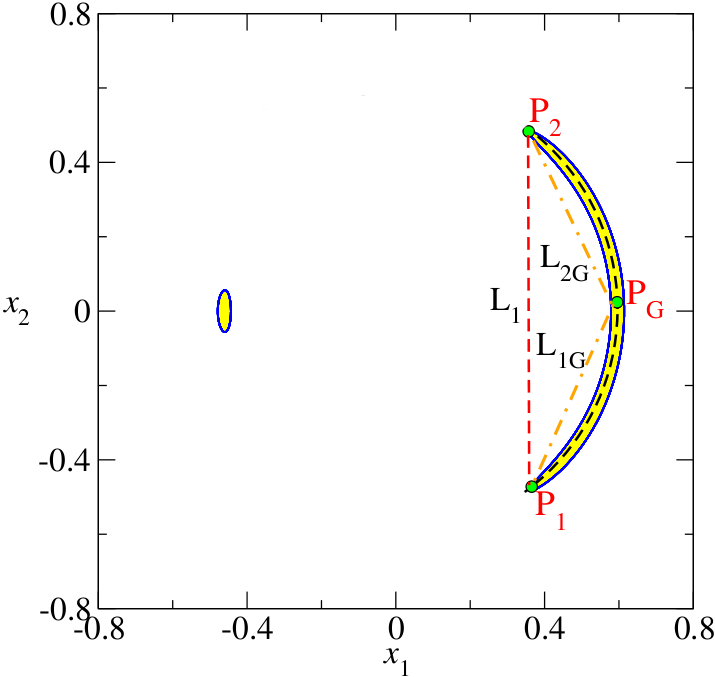
\includegraphics{graphics/measure_arc2.png}}
\hspace{3.cm}
\subfigure{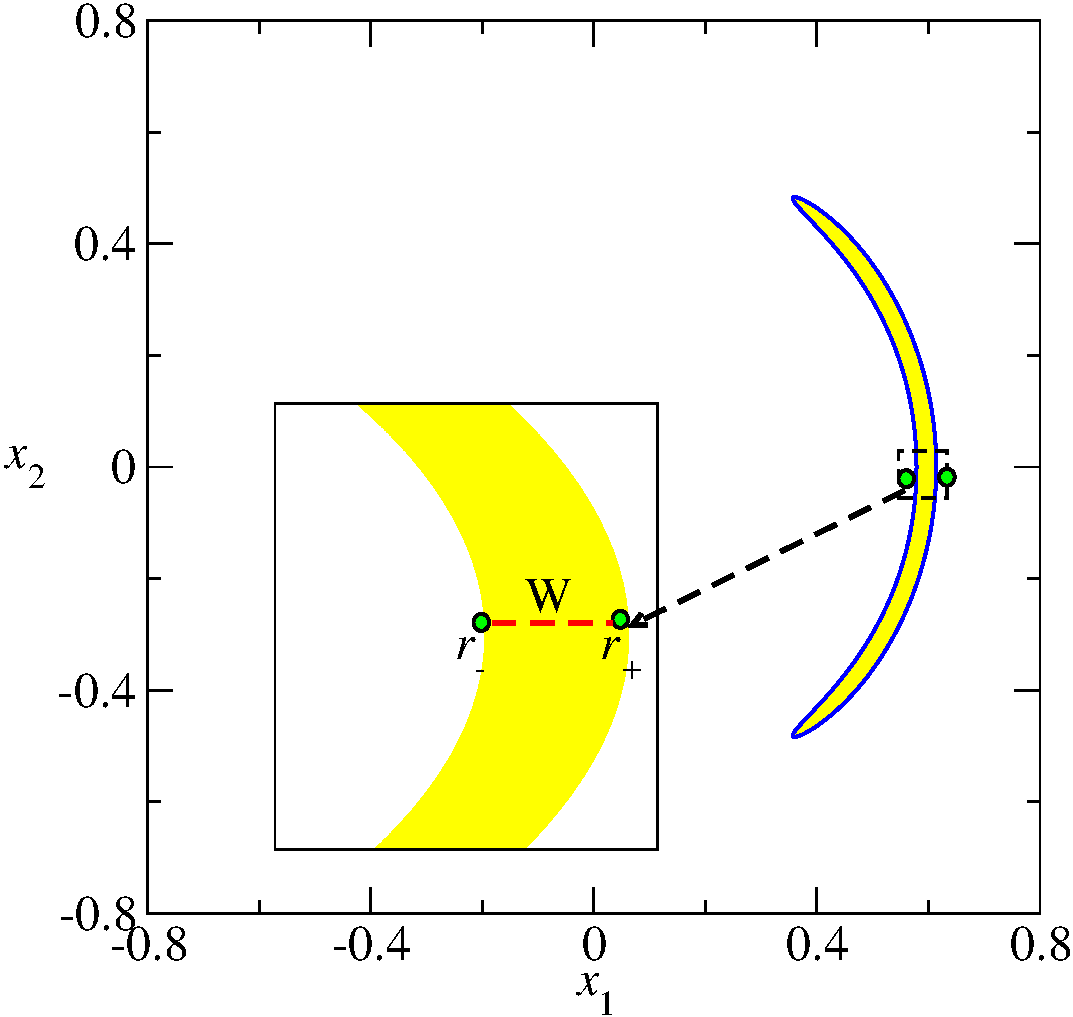
\includegraphics{graphics/measure_arc_w.pdf}}}
\caption{\label{measure_arcs} Method used to measure the length
and width of the images. Left Panel: Schematic representation for the
measurement of the length. Right Panel: Schematic representation for the
measurement of the width}
\end{figure*}


Following P.~Ferreira's ideas, shown in \cite{pedrothesis}, we will now
provide expressions for the measurements of the Length, Width and area
of the arc-images. Basically, Ferreira shows three methods for
measuring the length of the arcs, denoted $L_1$, $L_2$ and $L_3$, and
two methods for measure the width of the arcs, denoted $W$ and $W_q$.
The first method is overly simplistic and will not be considered in
this report, except to introduce the geometry of the arcs. We will
adapt the second and third methods in the framework of the
Perturbative Method and also to propose a method similar to C.~De Bom's
Method \cite{clecio} to measure the length.


In the Perturbative Method, the inner and outer radial vector of an arc
are given by

\bea
\vec{r}_{+}&=&(\re + x_{+})\cos{\te}\hat{\imath}+(\re
+x_{+})\sin{\te}\hat{\jmath}\label{rplus}\\
\vec{r}_{-}&=&(\re + x_{-})\cos{\te}\hat{\imath}+(\re
+x_{-})\sin{\te}\hat{\jmath}\label{rminus}
\eea
where $x_{\pm}$ are given by eq.~(\ref{elliptical_contour2}) for an
elliptical source oriented in any direction with respect to the source
potential semimajor axis.  Therefore, we may define a mean value of
the radial coordinate at a given angle $\te$ as

\bea
\bar{r}(\te)&=&\dfrac{r_{+}+r_{-}}{2}=\re+\left(\dfrac{x_{+}+x_{-}}{2}
\right) \nonumber \\
       &=& \re +\dfrac{1}{\kt}\left\{ \bar{f}_{1}(\theta) +%
\frac{\eta_s\sin(2\tilde{\theta})}{S}\left(\frac{1}{\re}\dfrac{\partial%
\bar{f}_0(\theta)}{\partial \theta}\right) \right\},\label{r_mean}
\eea
and the width as a function of $\te$ is given by 
\beq
W(\te)=x_+ - x_- = \dfrac{2}{\kt\,S}\sqrt{SR_{0}^2 -(1-\eta_s^2)\left[
\frac{1}{\re}\frac{\partial \bar{f}_0(\theta)}{\partial \theta}\right]^2}
\label{w_arc}
\eeq

Another useful quantity is the angle defining the barycenter of the image, given
by
\beq
\te_G={ \te_i+\te_f \over 2}
\label{angle_bary}
\eeq

where $ \te_i , \te_f $ label the beginning and ending angular position of a
given arc.

\subsection{Measurement of the Length}

The first method for arc length measurement, $L_1$, corresponds to the
distance between the points of the extrema of the arc and is
represented by the straight line segment joining the points $P_1$ and
$P_2$ (see Left Panel in Fig.~\ref{measure_arcs}).  By the condition
of the formation of images, we know the angles between which the arc
is formed. We call these angles as $\te_{i}$ and $\te_{f}$, and we
define the points $P_1$, $P_2$ as the mean radial vector at these
angles, i.e,

\beq
P_1=(\bar{r}_i\cos{\te_i},\bar{r}_{i}\sin{\te_i}), \quad
P_2=(\bar{r}_f\cos{\te_f},\bar{r}_{f}\sin{\te_f})
\eeq
where $\bar{r}_i\equiv \bar{r}(\te_i)$ and $\bar{r}_f\equiv \bar{r}(\te_f)$.
Then, the first measure for the length $L_1$ is
\beq
L_1=\sqrt{\bar{r}_i^2+\bar{r}_f^2-2\bar{r}_i\bar{r}_f\cos{(\te_f-\te_i)}}.
\label{first_length_def}
\eeq

This overly simplistic method was only introduced for notational
purposes, and will not be further discussed in this report.

The second method consists of calculating the distance resulting of
the summation of the straight line segments joining the points $P_1$
and $P_G$ ($L_{1G}$) and $P_G$ and $P_2$ ($L_{2G}$). Where the Point
$P_G$ correspond to the barycenter (i.e. gravicenter) of the image,
defined by radial vector at the angle $\te_G$.

\beq
P_G\equiv
(\bar{r}_G,\te_G)=(\bar{r}(\te_G)\cos{\te_G},\bar{r}(\te_G)\sin{\te_G})
\eeq

With the expression above, we have
\bea
L_{1G}&=&\sqrt{\bar{r}_i^2+\bar{r}_G^2-2\bar{r}_i\bar{r}_G\cos{
(\te_G-\te_i) } }\\ 
L_{2G}&=&\sqrt{\bar{r}_f^2+\bar{r}_G^2-2\bar{r}_i\bar{r}_G\cos{(\te_f-\te_G)}}
.\\
L_2&=&L_{1G}+L_{2G}
\eea

The third method consists of obtaining the equation of the circle
passing through three points belonging to the arc. Recall that that
the equation of a circle, with center ($x_{c},y_{c}$) and radius $R_c$
is
\begin{equation*}
 (x-x_c)^2+(y-y_c)^2=R^2_c
\end{equation*}
or
\beq
x^2+y^2+Ax+By+C=0\\
\eeq 

Considering the circular arc that passes through three points $P_1$, $P_G$ and
$P_2$, we need to solve the following system of equations


\begin{equation}
 \left[\begin{array}{c c c}
        \bar{r}_i\cos{\te_i} & \bar{r}_i\sin{\te_i} & 1\\
	\bar{r}_G\cos{\te_G} & \bar{r}_G\sin{\te_G} & 1\\
	\bar{r}_f\cos{\te_f} & \bar{r}_f\sin{\te_f} & 1\\
\end{array} \right]\left(\begin{array}{c} A \\ B\\ C
\end{array}\right)=-\left(\begin{array}{c}                         
\bar{r}^2_i\\ \bar{r}^2_G\\ \bar{r}^2_f\end{array}  \right) 
\end{equation}

where 
\bea
 x_c &=& -\dfrac{A}{2},\quad y_c = -\dfrac{B}{2}\\
 R_c &=&\sqrt{x_c^2+y_c^2-C}. 
\eea

The length of the image is then defined in this method by
\beq
L_3=R_c\arccos{\left(1-\dfrac{L_1^2}{2R_c^2}  \right)}
\eeq
where $L_1$ was given in Eq.~(\ref{first_length_def}).

Another proposal to measure the length yields perhaps a yet more
accurate way of obtaining it.  This method gives the length of a
circular arc segment passing through the points $P_1$ and $P_2$, see
the dashed line at the Left Panel of the Fig.~\ref{measure_arcs}, and
is given by

\beq
L_4=\int_{\te_i}^{\te_f}\bar{r}(\te)d\te.
\eeq

As a particular case, for the elliptical source contours aligned to the main
axis, we can obtain an analytic expression for the length of the arcs. For an
angle $\te$, we define
\beq
\mathcal{L}(\te)=\re\te+\mathcal{L}_s(\te)+\mathcal{L}_{\psi}(\te),
\eeq
where
\bea
\mathcal{L}_s&=&\frac{1}{\kt}\sqrt{\dfrac{1-\eta_s}{2\eta_s}}\left\{%
x_0\tan^{-1}{\left[\dfrac{\sqrt{2\eta_s}\sin{\te}}{\sqrt{1-\eta_s}}\right]}-%
y_0\tanh^{-1}{\left[\dfrac{\sqrt{2\eta_s}\cos{\te}}{\sqrt{1+\eta_s}}\right]}
\right\}\label{L_s}\\
\mathcal{L}_{\psi}&=&\frac{1}{\kt}\int\left\{f_{1}(\theta) +%
\frac{\eta_s\sin(2\theta)}{S}\left(\frac{1}{\re}\dfrac{\partial%
f_0(\theta)}{\partial \theta}\right)\right\} \label{L_psi}.
\eea



Then, using the expressions above we have
$L_4=\mathcal{L}(\te_f)-\mathcal{L}(\te_i)$.


Note, that for a circular source, $\mathcal{L}_s$ becomes

\beq
\mathcal{L}_s=\frac{x_0}{\kt}\sin{\te}-\frac{y_0}{\kt}\cos{\te}.
\eeq

\subsection{Measurement of the Width}

The first method to obtain the width of the arcs, is to measure the width 
at the angle $\te_G$, i.e, $W_q \equiv W(\te_m)$, using \eqref{w_arc}).


The second method consists of using the area of the image. This area is given by
\bea
\mathcal{A}&=&\int_{\te_i}^{\te_f}\int_{r_{-}(\te)}^{r_{+}(\te)}r \, dr \, d\te
\nonumber\\
           &=&\int_{\te_i}^{\te_f}W(\te)\bar{r}(\te)d\te.
\eea
where, $\bar{r}(\te)$ and $W(\te)$ are given by the Eqs. (\ref{r_mean}) and
(\ref{w_arc}) respectively.

Now we assume that the area of an arc is exactly that of a distorted
ellipse. With this assumption, the width of an arcs is given by
\beq
W_k=\dfrac{4\mathcal{A}}{\pi L_k}
\eeq
where $L_k$ corresponds to the one of the methods of measuring the length of the
arcs, $k=2,3$ or
$4$. 


\section{Inverse Modelling}

The perturbative method has the advantage of offering a linear non-parametric
approach for gravitational lensing. The key point is the reconstruction of the
fields $f_0(\te)$ and $f_1(\te)$.


For a circular source contour, a radial line of direction $\te$ intersects
the arc contours at two points, $r_i=\re+x_i$ and $r_o=\re+x_o$ (the inner part
and
the outer part). Now, we will use Alard Eq. 12

\beq
x = \frac{1}{\kappa_2}\left[ \overline{f}_{1}(\theta) \pm \sqrt{R_0^2 - \left(
\frac{1}{\re}\frac{\partial \overline{f}_0(\theta)}{\partial \theta} \right)^2}
\right]. \;\;\;
\eeq

And the separate two solutions for the inner and outer edges of the arc:


\bea
x_i = \frac{1}{\kappa_2}\left[ \overline{f}_{1}(\theta) - \sqrt{R_0^2 -%
\left( \frac{1}{\re}\frac{\partial \overline{f}_0(\theta)}{\partial \theta}
\right)^2} \right]. \;\;\;  \\
x_o = \frac{1}{\kappa_2}\left[ \overline{f}_{1}(\theta) + \sqrt{R_0^2 - %
\left( \frac{1}{\re}\frac{\partial \overline{f}_0(\theta)}{\partial \theta}
\right)^2} \right]. \;\;\;
\eea


With these, clearly

[There is a problem here, dealing with the definition of $r_{i,o}$ vs. $x_{i,o}$
-MSSG, Dec 6]
\beq
x_o + x_i  = {2 \over \kappa_2} \fbar -2\re
%= r_o+r_i - 2\re  ??
\eeq

And solve for $\fbar$:


\beq
\fbar = {\kappa_2 \over 2} (x_o+x_i) -2\kappa_2 \re
\eeq

which is exactly Alard eq. 29a, with his additional constant ($C=-\kt\re$).

Now take

\beq
x_o - x_i = {1 \over \kappa_2} \left(2 \sqrt{R_0^2 - {\left( {1 \over \re} \dfdt
\right)}^2 }\right)
\eeq

And solve for $\dfdt$ (few straight steps of algebra here):

\beq
\dfdt = \re \sqrt{R_0^2 - {\kappa_2^2 \over 4} (x_o-x_i)^2 }
\eeq

which is our form of Alard eq. 29b.

\section{Errors on arcs}
%%%%%%%%%%%%%%%%%%%%%%%%%%%%%%% Marcos

Recall that $\phi=\phi_0+\eps\psi$ and expand only $\psi$:

\beq
\phi=\phi_0+\eps\sum_{n=0}^{\infty}f_n(\theta)(r-\re)^n
\eeq

Differentiating we obtain

\bea
\frac{\partial \phi}{\partial r
}&=&\phi_0^\prime+\eps\sum_{n=1}^{\infty}f_n(\theta)n(r-\re)^{n-1} \\
\frac{\partial \phi}{\partial \theta}&=&\eps\sum_{n=0}^{\infty} \frac{\partial
f_n}{\partial \theta}(r-\re)^n
\eea

Evaluating at the Einstein radius $r=r_{\mathrm{E}}$, we have

\bea
\frac{\partial \phi}{\partial r }&=&\phi_0^\prime+f_1(\theta) \\
\frac{\partial \phi}{\partial \theta}&=&\eps \frac{\partial f_0}{\partial
\theta}
\eea

On the other hand, evaluating Eqs. 19 in Alard at $r=\re$, and using Eq. 16 in
Alard $\phi_0^\prime=1+2C_2(r-r_{\mathrm{E}}+...$

\bea
\frac{\prtl \phi}{\prtl r}&=& \phi_0^\prime -%
  \eps g(\te)\left[\phi_0^\prime+ \phi_0^{\prime
\prime}\right]=\phi_0^\prime-\eps g(\te)(1+C_2)\\
\frac{\prtl \phi}{\prtl \te}&=&-\eps\phi_0^\prime \frac{dg(\te)}{d\te}
\eea

Comparing these equations, we have a relation between the $f_n(\te)$ and
$g(\te)$ functions:

\bea
f_1&=&-(1+2C_2)g \\
\frac{df_0}{d\theta}&=&-\frac{dg}{d\theta}
\eea

Eq. (30) in Alard (to be derived later) is

\beq
dr=\frac{1}{\kappa_2}\left[ f_1+\frac{d^2f_0}{d\theta^2} \right]
\eeq

and in this case we have

\beq
dr=\frac{1}{\kappa_2}\left[ -(1+2C_2)g+\frac{d^2g}{d\theta^2} \right]
\eeq

Not sure what the effective parameter $dr_c$  in Eq 22 is and how to get it.
Assuming it's correct, i.e.
\beq
dr_c\sim -\frac{d^2g}{d\te^2}-2g
\eeq
we have that for e.g. the NFW profile with ellipticity (as in Eq. 28 of Alard)

\bea
\phi_0(q)&=&\frac{1}{2}\log^2\left(\frac{q}{2}\right)-2\arctan^2\left(\sqrt{
\frac{1-q}{1+q}}\right) \\
q&=&u_0r\sqrt{1-\eta\cos(\theta)}\approx u_0 r
\left[1-\frac{\eta}{2}\cos(2\theta)\right]
\eea

So in this case we have (notice $\eta/2$ plays the role of $\eps$ here, so only
expect expansion to work
for small ellipticities)

\bea
g(\te)&=&\frac{\eta}{2}\cos(2\theta) \\
\frac{d^2g(\te)}{d\te^2}&=&-2\eta\cos(\theta)=-4g
\eea

so that $dr_c=\eta\cos(\theta)$. Not sure if this is true for any elliptical
potential or if it's specific to NFW.
In any case the deviation is maximum for $\te=0,\pi$

If the Taylor expansion converges, truncating it at some order has a maximum
error given by the next order
term. In this case the maximum error due to the non-linearity of the gradient of
the potential is

\beq
D=3C_3\max[dr_c^2]=3C_3\eta^2
\eeq

Notice it increases with the ellipticity squared. For a general potential of the
form

\beq
\phi=\frac{1}{\alpha}r^{\alpha[1+\beta(r-1)]}
\eeq

we have

\beq
C_3=\frac{d^3\phi}{dr^3}|_{r=1}=-\frac{(\alpha-1)}{6}+\frac{\beta}{2}
\eeq

and $D^2$ follows.





\chapter{Description of the effect of perturbative fields on arcs}

Insert a motivation

\section{Pseudo-Elliptical Models}
The Pseudo-Elliptical models come from the distortion of the lensing potential, in which
the radial coordinate $r$ is replaced by $\xi$, i.e $\phi(r)\rightarrow \phi(\xi)$, where
\bea
\xi &=&r_0\,x_\eta=r_0\sqrt{x^2_{1\eta}+x^2_{2\eta}} \label{pe_cord} \\
x_{1\eta}&=&\sqrt{\ae} x_1\\
x_{2\eta}&=&\sqrt{\be} x_2
\eea
where $r_0$ is a model-dependent scaling parameter, and $\ae$, $\be$ are axes lengths for different parameterizations of the ellipticity.

The most common parameterizations for the ellipticity are

\begin{eqnarray}
\ae=1-\eta, &\qquad& \be =1+\eta \label{par_gk}\\
 \ae=1-\eta, &\qquad & \be =\dfrac{1}{1-\eta} \label{par_gen}\\
 \ae=1, &\qquad & \be =\dfrac{1}{(1-\eta)^{2}} \label{par_kee}
\end{eqnarray}

where \eqref{par_gk}) corresponds to the parametrization of the Angle Deflection
Model ($\eta=\varepsilon$ following the notation of \cite{golsekneib}),
\eqref{par_gen}) corresponds to the standard parametrization
($\eta=\varepsilon_\varphi$ following the notation of \cite{meneg}), and 
\ref{par_kee} corresponds to the Keeton's parametrization.

Working in polar coordinates $x_1=x\cos{\te}$ , $x_2=x\sin{\te}$ we obtain

\beq
\xi=r\sqrt{\ae \cos^2{\te}+\be\sin^2{\te}}.
\label{pe_radius}
\eeq

Regarding the Perturbative Approach, we can write any Pseudo-Elliptical Model as

\beq
\phi_{_\mathrm{PE}}(r)=\phi_0(r)+\phi(\xi)-\phi_0(r), \quad \psi_{_\mathrm{PE}}(r)=\phi(\xi)-\phi_0(r).
\label{pe_model}
\eeq

Here, we use the following notation

\begin{eqnarray*}
\phi_\xi\equiv \phi(\xi), &\quad&  \phi^\prime_\xi \equiv \dfrac{d\phi(\xi)}{d\xi}, \quad \phi^{\prime\prime}_\xi \equiv \dfrac{d^2\phi(\xi)}{d\xi^2}\\
\phi_0\equiv \phi(r),&\quad&  \phi^\prime_0 \equiv \dfrac{d\phi(r)}{dr}\\
\xer \equiv \re \sqrt{\ae \cos^2{\te}+\be\sin^2{\te}},&\quad& \scriptg(\eta,\te)=\re^2\mathcal{A}(\eta)\sin{(2\te)},\quad \mathcal{A}(\eta)=\be-\ae
\end{eqnarray*}

Now we derive the analytical expression for the main fields of the
Perturbative Method. Using the definition, we have

\beq
f_0(\te)=\phi(\xer)-\phi_0(\re)
\eeq
The derivative of $f_0$ with respect to $\te$ is
\beq
\frac{df_0}{d\te}=\dfrac{d\phi_{\xer}}{d\xer}\dfrac{d\xer}{d\te}=\frac{1}{2}\dfrac{\phi^\prime_{\xer}}{\xer}\scriptg(\eta,\te)
\label{df0_pe}
\eeq
where, we used 
\beq
\dfrac{d\xer}{d\te}=\frac{1}{2}\dfrac{\scriptg(\eta,\te)}{\xer}.                 
\label{dxer_pe}
\eeq

From Eqs.{(\ref{pe_radius}, \ref{pe_model})} we may obtain 

\begin{equation*}
\dfrac{\prtl \psi_{_{\mathrm{PE}}}(r) }{\prtl r}=\dfrac{d\phi_\xi}{d\xi}\dfrac{\prtl \xi}{\prtl r}-\dfrac{\prtl \phi_0}{\prtl r}
\end{equation*}

Evaluating this at the Einstein Radius, we have
\beq
f_1(\te)=\dfrac{\xer}{\re}\phi^\prime_{\xer}-\phi^\prime_0
\label{f1_pe}
\eeq

Also, taking the derivative of Eq.~(\ref{df0_pe}) respect to $\te$, it is straightforward to get
\beq
\dfrac{d^2f_0}{d\te^2}=\frac{1}{2}\scriptg_\te(\eta,\te)\dfrac{\phi^\prime_{\xer}}{\xer}+%
\frac{1}{4}\left[ \dfrac{\scriptg(\eta,\te)}{\xer}\right]^2\left(\phi^{\prime\prime}_{\xer}-\dfrac{\phi^{\prime}_{\xer}}{\xer}  \right)
\label{ddf0_pe}
\eeq
where $\scriptg_\te(\eta,\te)\equiv d\scriptg(\eta,\te)/d\te$.

Now, to write the expression of $d^nf_0 \over d\te^n$ and $f_1$ as function of the lensing functions, we use some basic relationships valid for
any circular model

\bea
\phi^\prime &\equiv& \dfrac{d\phi(r)}{d r}=\alpha(r) \label{dphi}\\
\phi^{\prime\prime}&\equiv& \dfrac{d^2\phi(r)}{d r^2}=2\kappa(r)-\dfrac{\alpha(r)}{r}\label{ddphi}\\
\gamma(r)&=&\dfrac{\alpha(r)}{r}-\kappa(r) \label{shear_gen}
\eea

Using these relationships and $r$ is a dummy variable, we have for the main fields
\bea
\dfrac{df_0}{d\te}&=& \frac{1}{2}\dfrac{\alpha(\xer)}{\xer}\scriptg(\eta,\te) \label{df0_pe2}\\
f_1(\te)&=&\dfrac{\xer}{\re}\alpha(\xer)-\alpha(\re) \label{f1_pe2}
\eea
and further
\beq
\label{ddf0_pe2}
\dfrac{d^2f_0}{d\te^2}=\frac{1}{2}\scriptg_\te(\eta,\te)\dfrac{\alpha(\xer)}{\xer}-%
\frac{\gamma(\xer)}{2}\left[ \dfrac{\scriptg(\eta,\te)}{\xer}\right]^2 .
\eeq

\subsection{Expression for small values of the ellipticity}

Now, we expand the analytical expressions for the main fields 
Eqs.(\ref{df0_pe2}, \ref{f1_pe2}) in a Taylor Series around $\eta=0$. 
Is straightforward to verify that

\bea
\dfrac{df_0}{d\te}& \approx & \eta\alpha(\re)\re\sin{(2\te)} \label{df0_pe_appr}\\
f_1(\te)&\approx&-\eta \kappa(\re)\re\cos{(2\te)} \label{f1_pe_appr}
\eea

And from  Eq.~(\ref{df0_pe_appr}), or expanding Eq.~(\ref{ddf0_pe2}) in a Taylor Series, we obtain
to
\beq
\dfrac{d^2f_0}{d\te^2}=2\eta\alpha(\re)\re\cos{(2\te)} \label{ddf0_pe_appr}
\eeq

For example, if we consider the Pseudo-Elliptical SIS (setting $\re=1$) we get to the
Eqs.(17) of Alard's Paper 2008 (without considering the contribution of substructures), i.e,
\begin{eqnarray*}
 f_1(\te)&\approx&-\frac{\eta}{2}\cos{(2\te)}\\
 \dfrac{df_0}{d\te}& \approx & \eta\sin{(2\te)} 
\end{eqnarray*}
 


\pagebreak

\section{Elliptical Models } % Bruno
\subsection{General results for elliptical models}
Contrary to pseudo-elliptical models, elliptical models introduce the ellipticity directly into the convergence. To do this, we apply the following transformation to the convergence of an axisymetric model:
\beq
\label{variavel-eliptica}
x^2 \rightarrow \frac{x^2}{a^2} + \frac{y^2}{b^2}.
\eeq
It can then be shown that the derivatives of the potential in Cartesian coordinates can be written as (cf. Gabriel's master thesis):
\begin{eqnarray}
\label{der-pot1}
\phi_1(x_1,x_2) &=& abx_1J_0, \\
\label{der-pot2}
\phi_2(x_1,x_2) &=& abx_2J_1, \\
\label{der-pot3}
\phi_{11}(x_1,x_2)&=& 2abx_1^2K_0 + abJ_0, \\
\label{der-pot4}
\phi_{22}(x_1,x_2)&=& 2abx_2^2K_2 + abJ_1, \\
\label{der-pot5}
\phi_{12}(x_1,x_2)&=& 2abx_1x_2K_1,
\end{eqnarray}
where $\phi_i$ is the derivative of $\phi$ according to $x_i$ and $J_n$ and $K_n$ are defined as  
\begin{eqnarray}
\label{int-1}
J_n(r,\te)&=& \int_{0}^{1} \dfrac{\kappa\left( m(u) \right) }{\left[1-(1-b^2)u \right]^{\frac{1}{2}+n} \left[1-(1-a^2)u \right]^{\frac{3}{2}-n}}du,\\
K_n(r,\te)&=& \int_{0}^{1} \dfrac{u\kappa'\left( m(u) \right) }{\left[1-(1-b^2)u \right]^{\frac{1}{2}+n} \left[1-(1-a^2)u \right]^{\frac{5}{2}-n}}du,
\end{eqnarray}
In these integrals, $m$ is written as (in radial coordinates for our purposes)
\beq
m^2 = ur^2\left( \dfrac{cos^2\te}{1-(1-a^2)u} + \dfrac{sen^2\te}{1-(1-b^2)u}\right)\,.
\eeq
From the first-order derivatives in Cartesian coordinates, we can obtain the ones in polar coordinates using the transformation of the gradient
\bea
\frac{\partial\phi}{\partial r}&=&\phi_1\cos\,\te+\phi_2 \sin\,\te\\
\frac{\partial\phi}{\partial \te}&=&-\phi_1\sin\,\te+\phi_2\cos\,\te
\eea
Then it is easy to obtain
\bea
<<<<<<< HEAD
\frac{\partial \phi}{\partial
r}&=&abr\left[J_0(r,\te)cos^2\te+J_1(r,\te)sin^2\te\right]\\
\frac{\partial \phi}{\partial \te}&=&abr^2sin\,\te
cos\,\te\left[J_1(r,\te)-J_0(r,\te)\right]
\eea
In order to get the coefficients in Alard's expansion, we need to extract the
axisymmetric part of the potential. Defining
$\psi(r,\te)\equiv\phi(r,\te)-\phi_0(r)$, we arrive at
\bea
f_1&=&\re\left[ab\left(J_0(R_E,\te)\,cos^2\te+J_1(R_E,\te)\,sen^2\te\right)-1\right]\label{f1-sie}
\\[10pt]
\frac{{\rm d}f_0}{{\rm
d}\te}&=&ab\,\frac{\re^2}{2}\left[J_1(R_E,\te)-J_0(R_E,\te)\right]sen\,2\te\label{df0-sie}\\[10pt]
\frac{{\rm d}^2f_0}{{\rm
d}\te^2}&=&ab\,\re^2\Bigg\{\left[J_1(R_E,\te)-J_0(R_E,\te)\right]cos\,2\te +\nonumber\\ 
&&+\frac{\re^2}{2}\left[K_0-2K_1(R_E,\te)+ K_2(R_E,\te)\right]sen^22\te\Bigg\}\label{d2f0-sie}
\eea
\subsection{SIE: CC, caustics and deformation cross-section}

SIE models are the elliptical generalization of the SIS model. As such, the
convergence can be obtained using eq. (\ref{variavel-eliptica}):
\beq
\kappa_{SIE}(m)=\frac{R_E}{2m}\label{convergence-SIE}
\eeq
where $m$ is given by eq. (\ref{m}). In this case, it is possible to calculate
the integrals (\ref{Jn}) and (\ref{Kn}) analitically.
\bea
J_n(r,\te)&=&\frac{\re}{r}\frac{1}{\sqrt{\varepsilon_n+A(\theta)}}\tanh^{-1}
\left(\sqrt{\frac{\varepsilon_n+A(\theta)}{1+A(\theta)}}\right)
\eea
where
\bea
\varepsilon_0&=&1-a^2\\
\varepsilon_1&=&1-b^2\\
A(\theta)&=&b^2-1+(a^2-b^2)\cos^2\theta
\eea
It will be useful to express eqs. (\ref{Jn}) and (\ref{Kn}) in terms of the
ellipticity. Let us choose the prescription
$\left(a=(1-\epsilon)^{-1/2},\,b=(1-\epsilon)^{1/2}\right)$. Then
\bea
\bar{\varepsilon}_0&=&\frac{\epsilon}{\epsilon-1}\\
\bar{\varepsilon}_1&=&\epsilon\\
\bar{A}(\theta)&=&\epsilon\left[-1+\left(\frac{\epsilon-2}{\epsilon-1}
\right)\cos^2\theta\right]
\eea
and
\bea
J_0(r,\te)&=&\frac{R_E}{r}\frac{\tanh^{-1}\left[\frac{\sqrt{-\frac{(-2+\epsilon ) \epsilon  \text{Sin}[\theta ]^2}{-1+\epsilon }}}{\sqrt{1-\epsilon +\frac{(-2+\epsilon ) \epsilon  \text{Cos}[\theta ]^2}{-1+\epsilon }}}\right]}{\sqrt{-\frac{(-2+\epsilon ) \epsilon  \text{Sin}[\theta ]^2}{-1+\epsilon }}}\\[10pt]
J_1(r,\te)&=&\frac{R_E}{r}\frac{\tanh^{-1}\left[\frac{\sqrt{\frac{(-2+\epsilon ) \epsilon  \text{Cos}[\theta ]^2}{-1+\epsilon }}}{\sqrt{1-\epsilon +\frac{(-2+\epsilon ) \epsilon  \text{Cos}[\theta ]^2}{-1+\epsilon }}}\right]}{\sqrt{\frac{(-2+\epsilon ) \epsilon  \text{Cos}[\theta ]^2}{-1+\epsilon }}}\\[10pt]
K_0(r,\te)&=&\frac{R_E}{2r} \left(\frac{\text{Cot}[\theta ]^2}{\sqrt{1-\epsilon +\frac{(-2+\epsilon ) \epsilon  \text{Cos}[\theta ]^2}{-1+\epsilon }}}-\frac{\text{ArcTanh}\left[\frac{\sqrt{-\frac{(-2+\epsilon ) \epsilon  \text{Sin}[\theta ]^2}{-1+\epsilon }}}{\sqrt{1-\epsilon +\frac{(-2+\epsilon ) \epsilon  \text{Cos}[\theta ]^2}{-1+\epsilon }}}\right] \text{Csc}[\theta ]^2}{\sqrt{-\frac{(-2+\epsilon ) \epsilon  \text{Sin}[\theta ]^2}{-1+\epsilon }}}\right)\\[10pt]
K_1(r,\te)&=&-\frac{R_E}{2r \sqrt{1-\epsilon +\frac{(-2+\epsilon ) \epsilon  \text{Cos}[\theta ]^2}{-1+\epsilon }}}\\[10pt]
K_2(r,\te)&=&\frac{R_E}{2r} \left(-\frac{\text{ArcTanh}\left[\frac{\sqrt{\frac{(-2+\epsilon ) \epsilon  \text{Cos}[\theta ]^2}{-1+\epsilon }}}{\sqrt{1-\epsilon +\frac{(-2+\epsilon ) \epsilon  \text{Cos}[\theta ]^2}{-1+\epsilon }}}\right] \text{Sec}[\theta ]^2}{\sqrt{\frac{(-2+\epsilon ) \epsilon  \text{Cos}[\theta ]^2}{-1+\epsilon }}}+\frac{\text{Tan}[\theta ]^2}{\sqrt{1-\epsilon +\frac{(-2+\epsilon ) \epsilon  \text{Cos}[\theta ]^2}{-1+\epsilon }}}\right)
\eea
For small ellipticity, we can do a series expansion around $\epsilon=0$. At
linear order, this gives
\bea
J_0(R_E,\te)cos^2\te+J_1(R_E,\te)sin^2\te&=&\left(1-\frac{
\epsilon\cos\,2\theta}{2}\right)\\
J_1(r,\te)-J_0(r,\te)&=&\frac{2\epsilon}{3}
\eea
and
\bea
f_1&=&\\[10pt]
\frac{{\rm d}f_0}{{\rm
d}\te}&=&\\[10pt]
\frac{{\rm d}^2f_0}{{\rm
d}\te^2}&=&
\eea
\subsection{SIE: CC, caustics and arcs}
\subsection{ENFW: CC, caustics and arcs}
\section{Substructures}
\begin{wrapfigure}{r}{0.4\textwidth}
  \begin{center}
%  \centering{\epsfig{Fig_subsstructure.eps,width=0.45\textwidth}}
   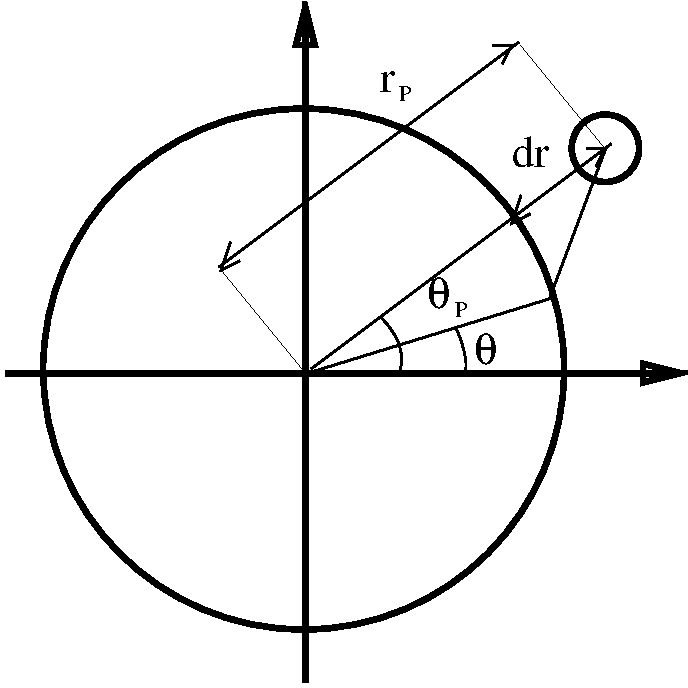
\includegraphics[width=0.30\textwidth]{graphics/Fig_subsstructure.pdf}
\label{fig:substruc}
  \end{center}
    \caption{Geometry of the perturbation induced by the substructure. The large circle corresponds to Einstein Ring,
  while the smaller one represents the substructure located at $r_p=\re +\zeta$.}
\end{wrapfigure}

We may consider the perturbation as
\begin{equation}
\psi_{ss}(r,\te,\pi_p)=\varphi(\zeta)
\end{equation}
where the ``ss'' indicates substructure, $\varphi$ corresponds to a central potential (any circular model, such as SIS, NFW and so on) and $\pi_p$
are the substructure parameters, such as mass, position and inclination angle. $\zeta$ comes from Fig. \ref{fig:substruc} (in which $dr=\zeta$)
where
\begin{eqnarray}
\vec{r}_p&=&r_p\cos{\tep}\hat{\imath} + r_p\sin{\tep}\hat{\jmath}\\
\vec{r}&=&r\cos{\te}\hat{\imath} + r\sin{\te}\hat{\jmath}\\
\vec{\zeta}&=&\vec{r}_p-\vec{r}.
\end{eqnarray}
Taking the modulus of $\zeta$, is straightforward to verify that
\begin{equation}
\zeta(r,\te)=\sqrt{r^2-2r r_p\cos{(\te-\tep)}+r^2_p}.
\label{xirte}
\end{equation}

Before giving the analytical expression for the fields $f_1$ and ${d^nf_0 \over d\te^n}$ ($n=1,2$), we
give some useful results (with $\zeta = \zeta(r,\te)$).
\begin{eqnarray}
\Omega(\zeta) & \equiv & r r_p \sin{(\te-\te_p)} \\
\dfrac{d\zeta}{d\te}&=&  \dfrac{\Omega(\zeta)}{\zeta}\\
\dfrac{d\Omega(\zeta)}{d\te}&=&r r_p\cos{(\te-\te_p)}\\
\dfrac{d\zeta}{dr}&=&\dfrac{r-r_p\cos{(\te-\te_p)}}{\zeta}
\end{eqnarray}

Introducing the following notation
\begin{eqnarray}
\varphi_\zeta & \equiv & \varphi(\zeta) \nonumber \\
\varphi^\prime_\zeta &=& d\varphi_\zeta \over d\zeta \nonumber  \\
\varphi^{\prime\prime}_\zeta &=& d^2\varphi_\zeta \over d\zeta^2 \nonumber 
\end{eqnarray}

and using the relations above we have

\begin{eqnarray}
\dfrac{\prtl \psi_{ss}}{\prtl \te}&=&\Omega(\zeta)\dfrac{\varphi^\prime}{\zeta}\label{df0}\\
\dfrac{\prtl^2 \psi_{ss}}{\prtl\te^2}&=&\left[\varphi^{\prime\prime}_\zeta-\dfrac{\varphi^\prime_\zeta}{\zeta}\right]%
\left(\dfrac{\Omega(\zeta)}{\zeta}\right)^2+[r r_p\cos{(\te-\tep)}]\dfrac{\varphi^\prime_\zeta}{\zeta}\label{ddf0}\\
\dfrac{\prtl \psi_{ss}}{\prtl r}&=&[r-r_p\cos{(\te-\tep)}]\dfrac{\varphi^\prime_\zeta}{\zeta}\label{f1}
\end{eqnarray}

Using the Eqs.~(\ref{dphi}, \, \ref{ddphi} and \ref{shear_gen}), where $r$ is dummy variable, we can define 
$\al_\zeta=\al(\zeta)=\varphi^\prime_\zeta$, $\kappa_\zeta=\kappa(\zeta)$ and $\gamma_\zeta=\al_\zeta/\zeta-\kappa_\zeta$. 
From Eqs.(\ref{xirte}, \ref{df0}-\ref{f1}) (evaluated at $r=\re$), we obtain the analytical expressions for the main fields of
the perturbative approach as function of the angle deflection and convergence, i.e.
\begin{eqnarray}
\dfrac{df_0}{d\te}&=&\al_{\xie}\dfrac{\Omega(\xie)}{\xie}\\
% \dfrac{d^2f_0}{d\te^2}&=&2\left[\kappa_{\xie}-\dfrac{\al_{\xie}}{\xie}\right]%
% \left(\dfrac{\Omega(\xie)}{\xie}\right)^2+\al_{\xie}\dfrac{[\re r_p\cos{(\te-\tep)}]}{\xie}\\
\dfrac{d^2f_0}{d\te^2}&=& \al_{\xie}\dfrac{[\re r_p\cos{(\te-\tep)}]}{\xie}% 
- 2\gamma_{\xie} \left(\dfrac{\Omega(\xie)}{\xie}\right)^2\\
f_1(\te)&=&\al_{\xie}\dfrac{[\re-r_p\cos{(\te-\tep)}]}{\xie},
\end{eqnarray}

\subsection{SIS model as substructure}

As application of these analytical expressions, we will consider the case of the Singular Isothermal Sphere, for
which $\psi(r,\te,\pi_p)=m_p\zeta$, where $m_p$ is the mass contained within the critical radius.
Is very easy to verify that $\al_\zeta=m_p$,  $\kappa_\zeta=m_p/(2\zeta)$ (this expression comes from the usual
definition of the SIS convergence) and therefore we obtain
\begin{eqnarray}
\dfrac{d f_0}{d\te}&=&\dfrac{\re m_p r_p \sin{(\te -\tep)}}{\sqrt{\re^2-2\re r_p\cos{(\te-\tep)}+r^2_p}}.\\
f_1&=&\dfrac{m_p[\re-r_p\cos{(\te-\tep)}]}{\sqrt{\re^2-2\re r_p\cos{(\te-\tep)}+r^2_p}}.
\end{eqnarray}
If we choose $\re=1$ we get to the expression given in Alard's 2008 Paper .

Another quantity useful to calculate the critical and caustic lines is
\begin{equation}
\dfrac{d^2 f_0}{d\te^2}=\dfrac{m_p}{\sqrt{\re^2-2\re r_p\cos{(\te-\tep)}+r^2_p}}%
\left[\re r_p\cos{(\te-\tep)}- \dfrac{[\re r_p\sin{(\te-\tep)}]^2}{\re^2-2\re r_p\cos{(\te-\tep)}+r^2_p} \right].
\end{equation}

Conclusions: Now, we are able to at least consider substructure in the form of a circular lens.


\section{External Shear + Continuous Matter}

Objects near the main lens galaxy or along the line of sight often perturb the lensing potential.
In the case that we are considering the contribution of the mass distribution external to the lens,
we can work with the potential coming from the external mass + external shear.
\beq
\phi(r)=\phi_0(r)+\frac{r^2}{2}\left[ \kex-\gex\cos{2(\te-\te_\gamma)}\right].
\eeq
where the perturbative potential, in this case is
\beq
\psi_{_{\mathrm{EX}}}(r)=\frac{r^2}{2}\left[ \kappa_{_{\mathrm{EX}}}-\gamma_{_{\mathrm{EX}}}\cos{2(\te-\te_\gamma)}\right]
\eeq
From the expression above, is easy get to
\bea
f_1(\te)&=& \re\left[\kex-\gex\cos{2(\te-\te_\gamma)}   \right]\\
\dfrac{d f_0}{d\te} (\te)&=& \re^2\gex\sin{2(\te-\te_\gamma)}\\
\dfrac{d f^2_0}{d\te^2}(\te)&=& 2\re^2\gex\cos{2(\te-\te_\gamma)}\\
\eea

Note that this model for perturbation is the most simples, but don't forget that $\re$ depends on the
unperturbed potential, for example: could be NFW, SIS, Cuspy-NFW, etc etc. 

\section{Aplications to Deformation Arc Cross Section}
In this section we collect our results for the cross section for deformation
arcs. This include plot the constant distortion curves and the calculation of
the deformation arc cross section as a function of the lens parameters.

\subsection{SIEP model}

\begin{figure*}[!ht]
\resizebox{\hsize}{!}{
\subfigure{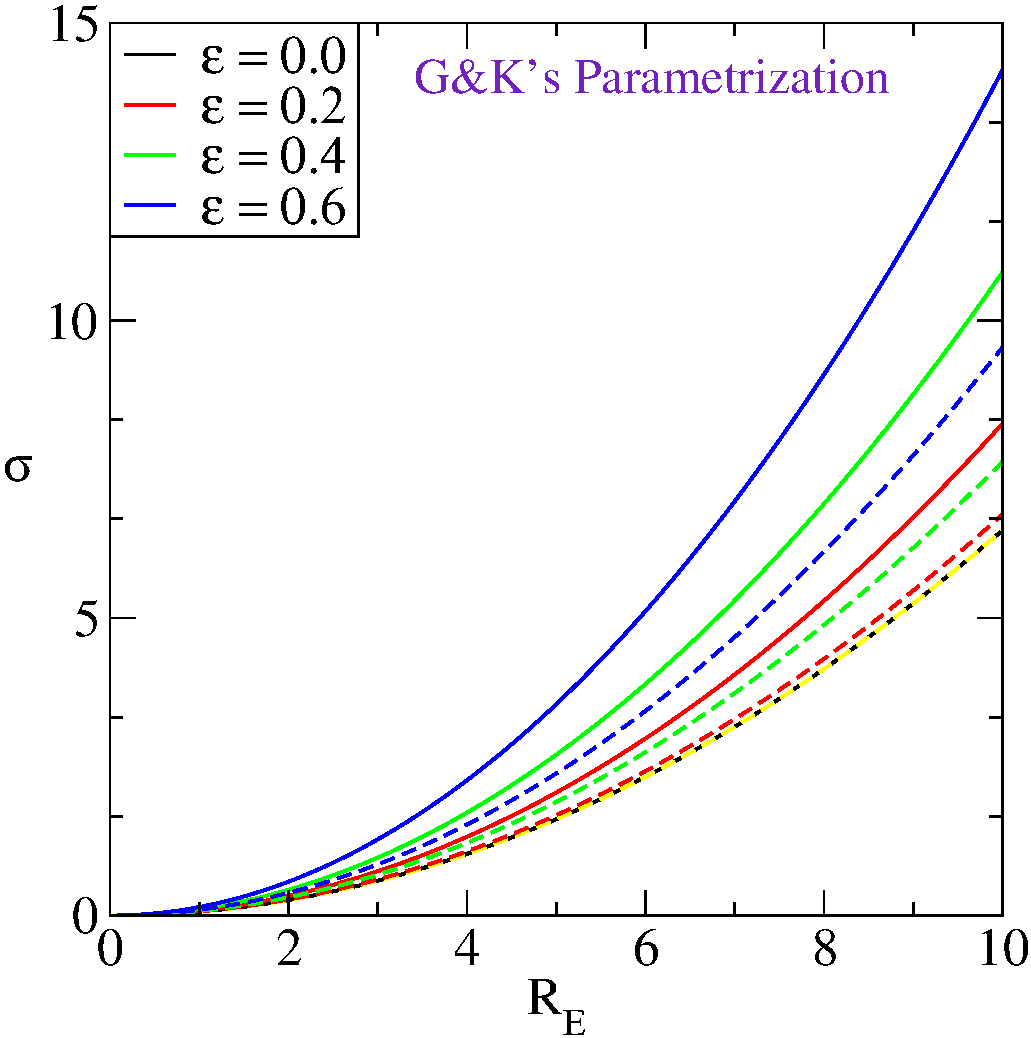
\includegraphics{graphics/dcs_siep_vs_re-gk_pm.pdf}}\hspace{1.cm}
\subfigure{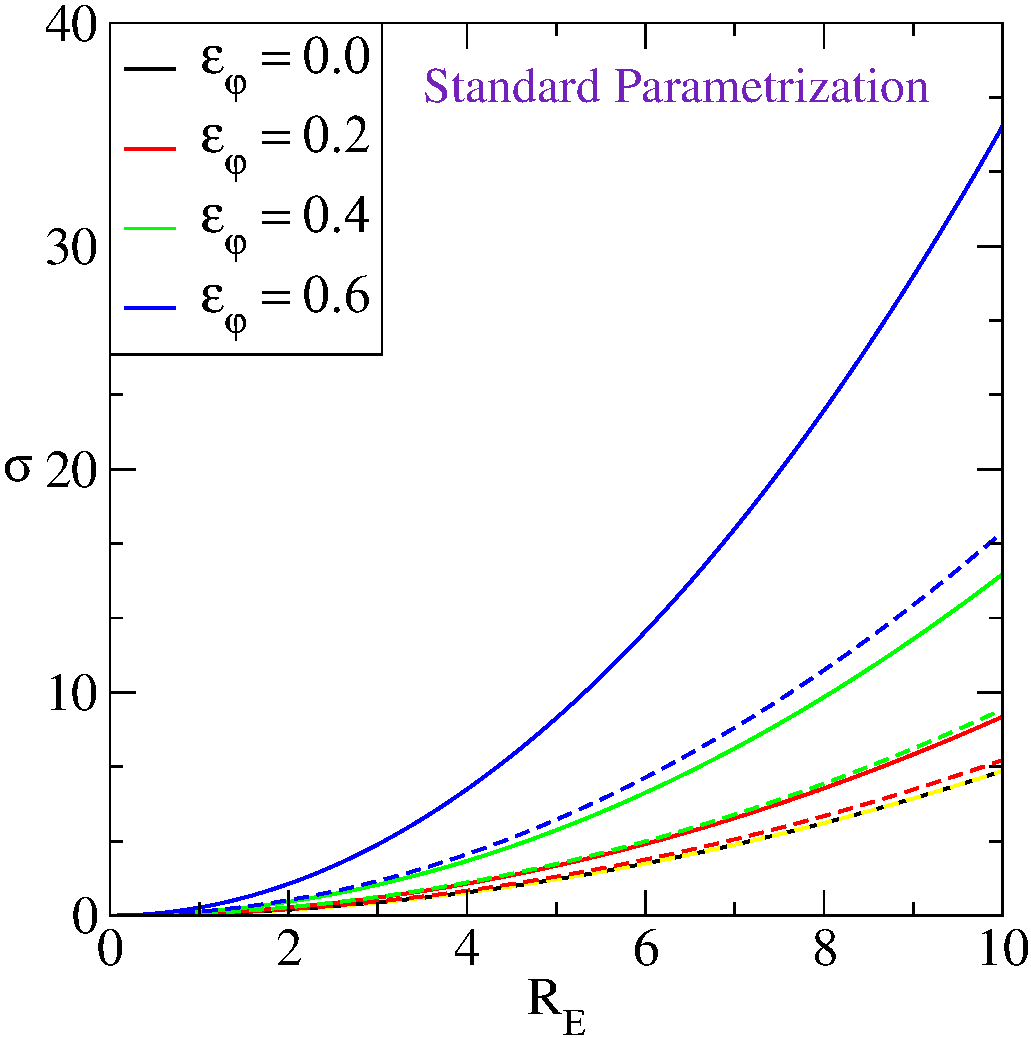
\includegraphics{graphics/dcs_siep_vs_re-st_pm.pdf}}\hspace{1.cm}
\subfigure{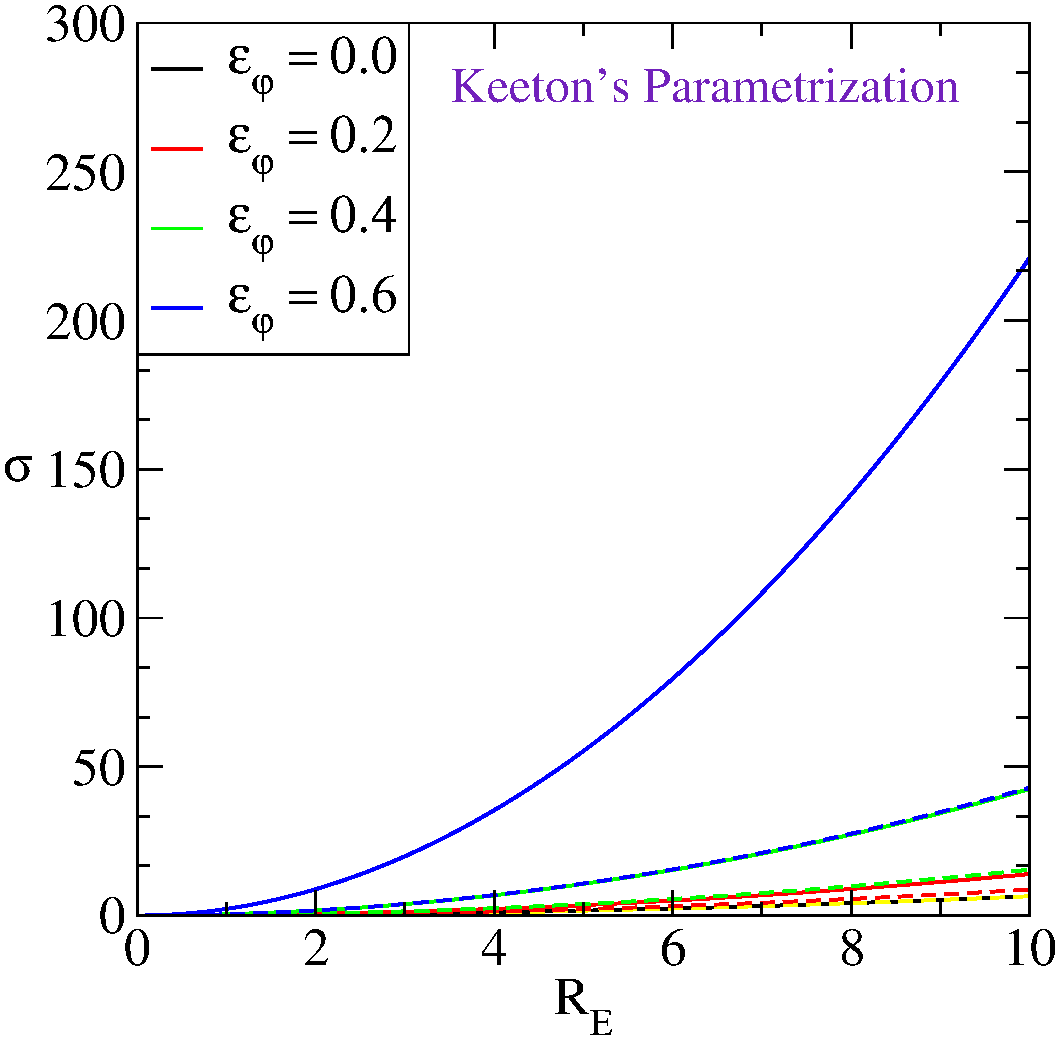
\includegraphics{graphics/dcs_siep_vs_re-k_pm.pdf}}}
\caption{\label{dcs_siep_re_pm} Deformation cross section for the  SIEP lensing
model as a function of $R_{\rm E}$. Solid Lines correspond to the Exact
Solution. Dashed-Lines correspond to Perturbative Approach (Yellow dashed-lines 
correspond to $\varepsilon.=0$). Left Panel:
Parametrization of the Angle Deflection Model. Middle Panel: Standard
Parametrization. Right Panel: The Keeton's parametrization.  The calculations
were done for $R_{\rm th}=10$.}
\end{figure*}

\begin{figure*}[!ht]
\resizebox{\hsize}{!}{
\subfigure{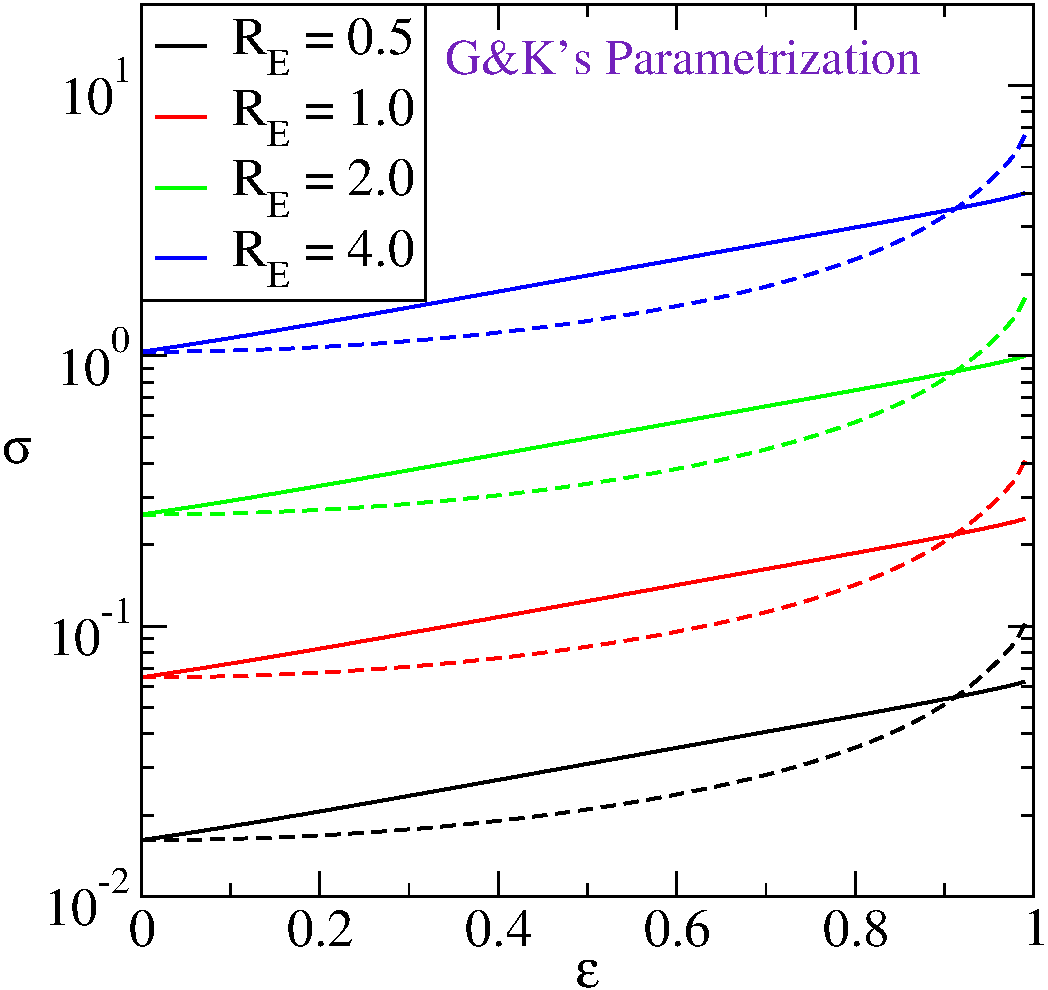
\includegraphics{graphics/dcs_siep_vs_e-gk_pm.pdf}}\hspace{1.cm}
\subfigure{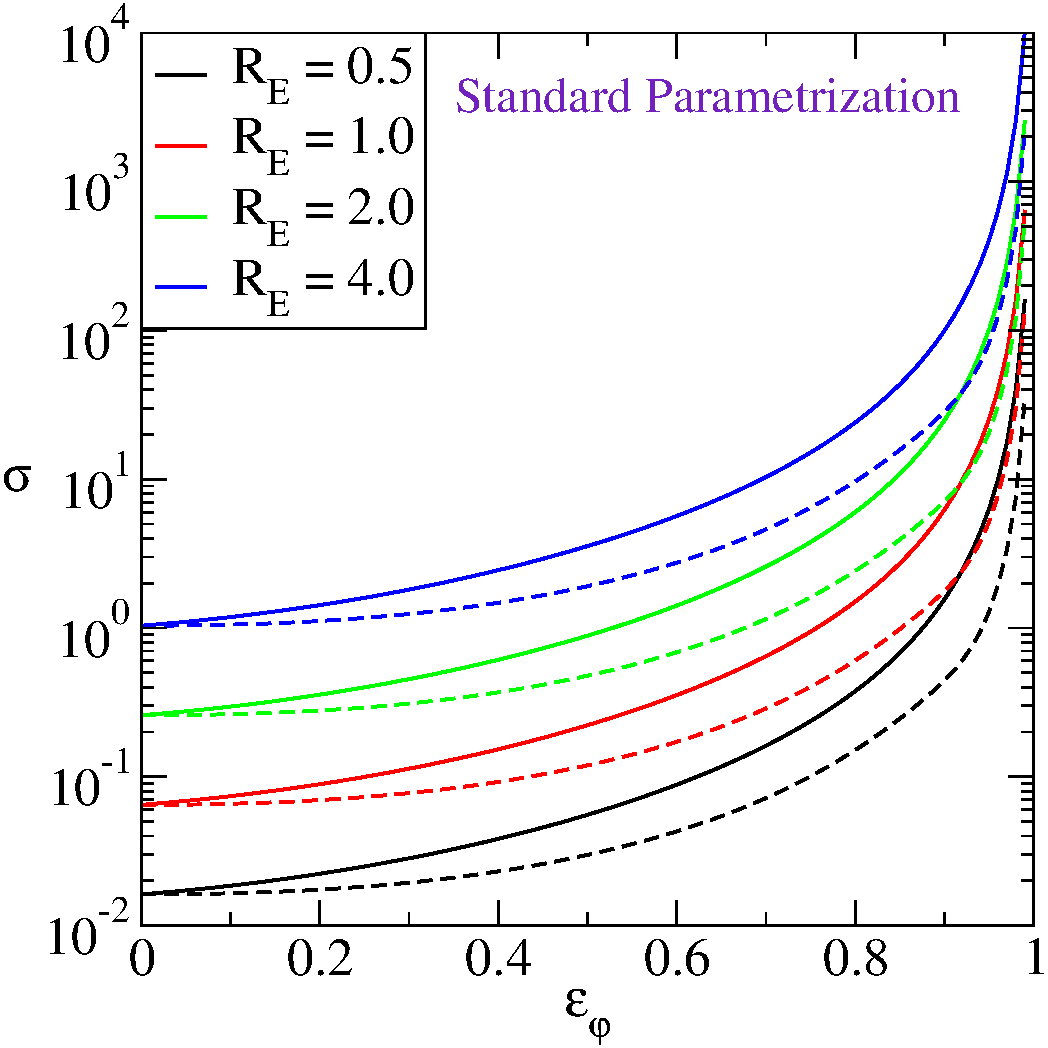
\includegraphics{graphics/dcs_siep_vs_e-st_pm.pdf}}\hspace{1.cm}
\subfigure{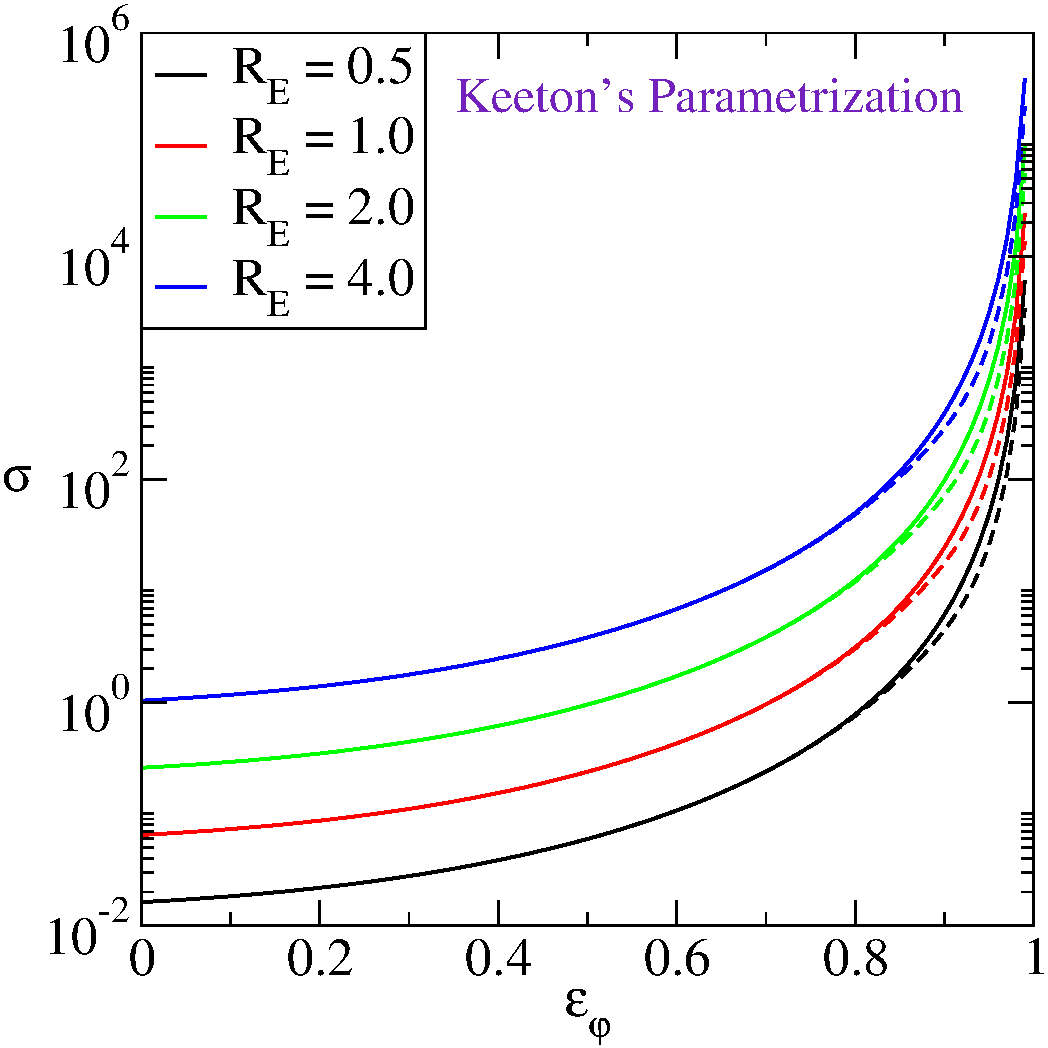
\includegraphics{graphics/dcs_siep_vs_e-k_pm.pdf}}}
\caption{\label{dcs_siep_e_pm} Deformation cross section for the  SIEP lensing
model as a function of the ellipticity. Solid Lines correspond to the Exact
Solution. Dashed-Lines correspond to Perturbative Approach. Left Panel:
Parametrization of the Angle Deflection Model. Middle Panel: Standard
Parametrization. Right Panel: The Keeton's parametrization. The calculations
were
made for $R_{\rm th}=10$.}
\end{figure*}

\begin{figure*}[!ht]
\resizebox{\hsize}{!}{
\subfigure{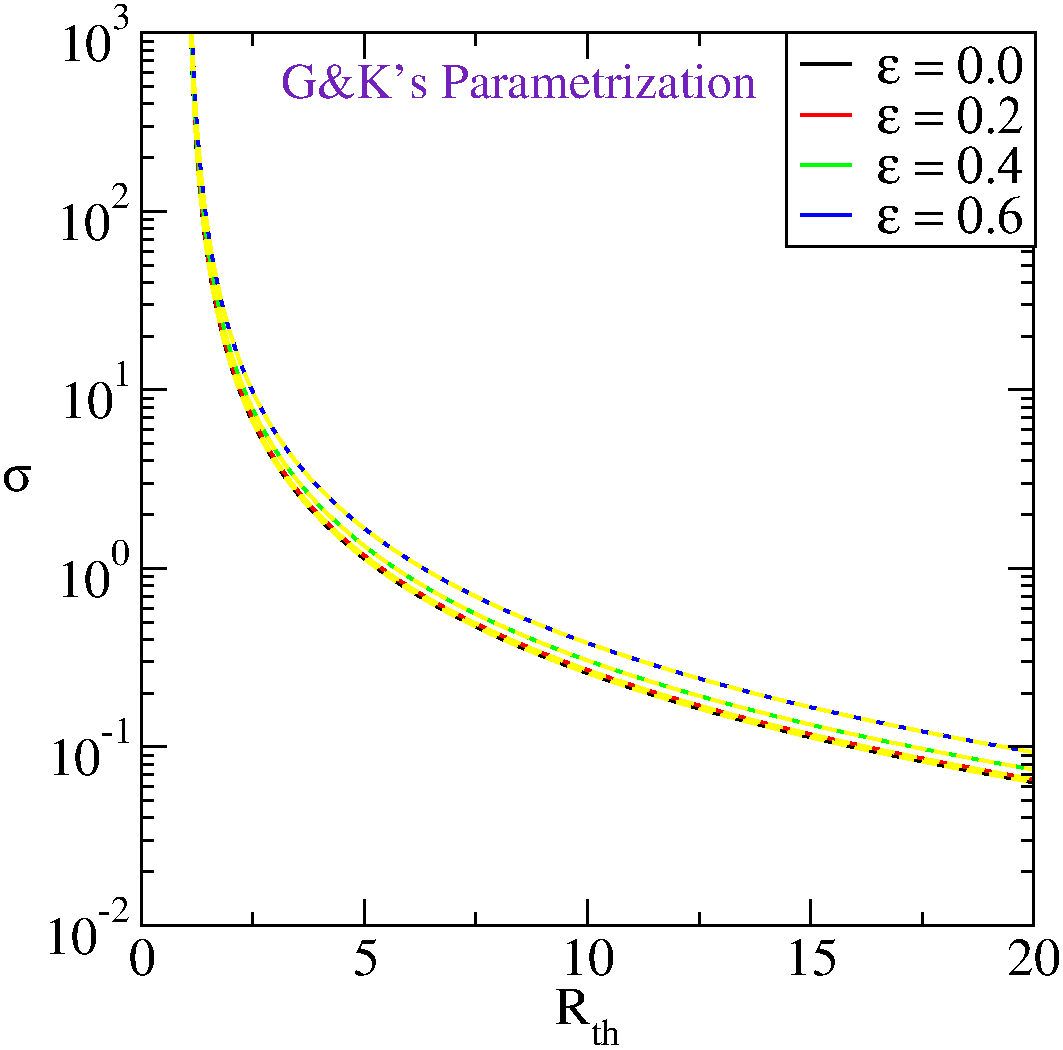
\includegraphics{graphics/dcs_siep_vs_rth-gk_pm.pdf}}\hspace{1.cm}
\subfigure{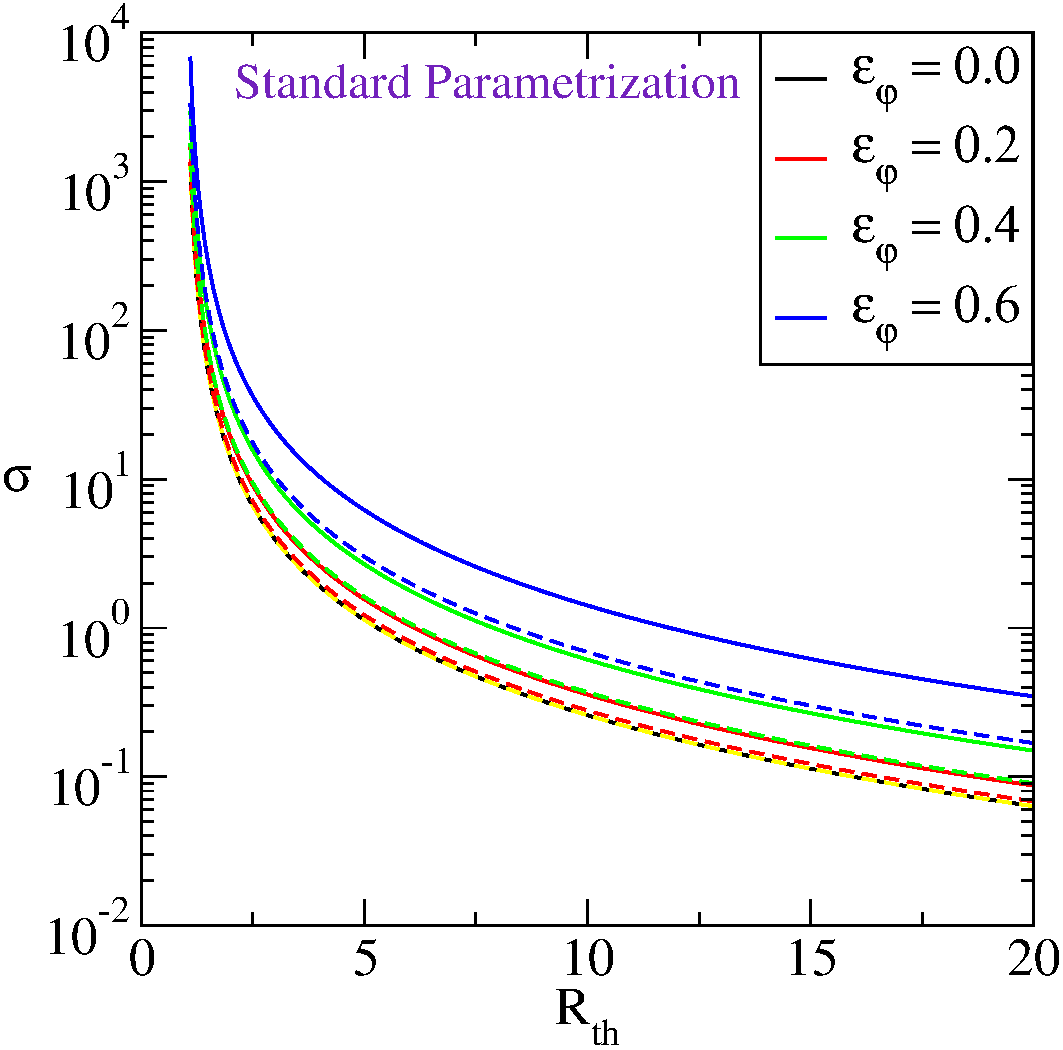
\includegraphics{graphics/dcs_siep_vs_rth-st_pm.pdf}}\hspace{1.cm}
\subfigure{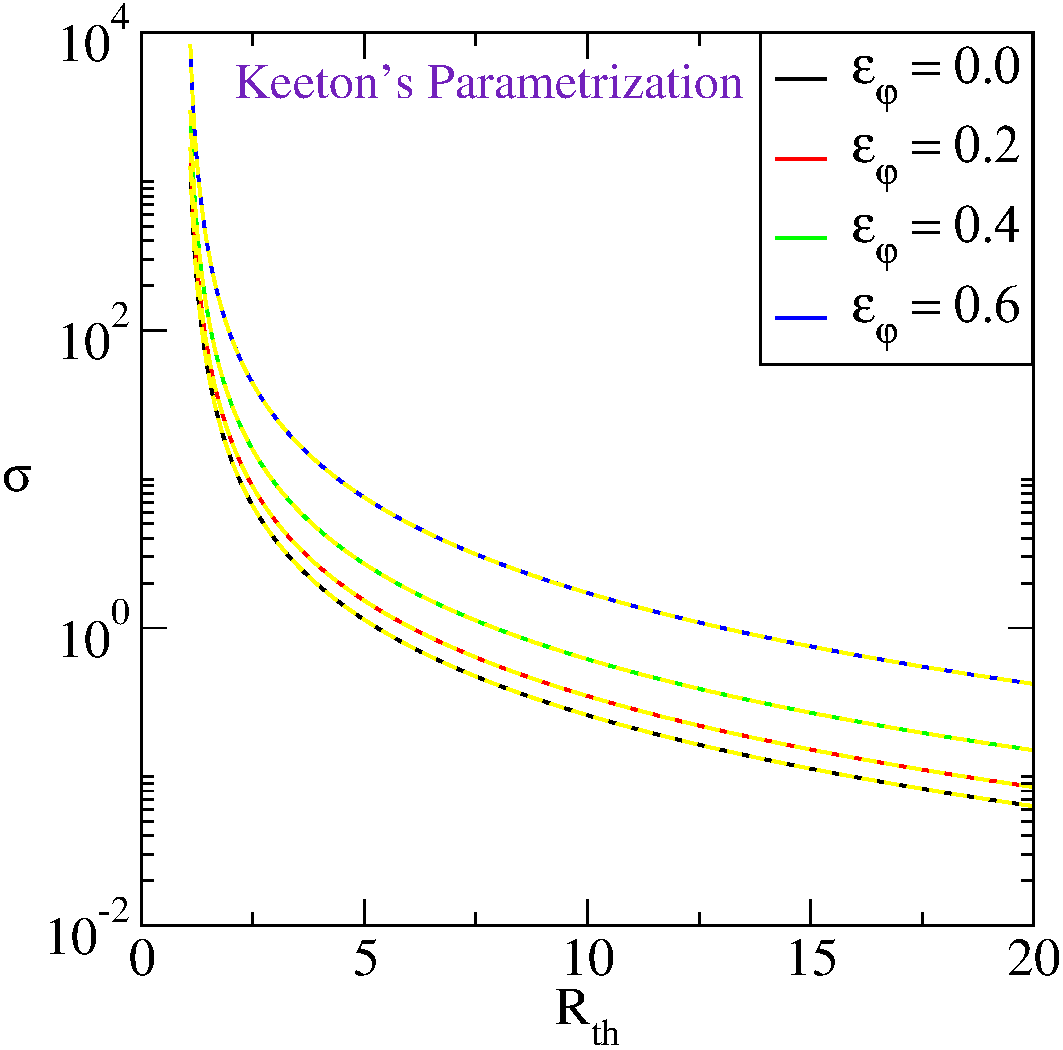
\includegraphics{graphics/dcs_siep_vs_rth-k_pm.pdf}}}
\caption{\label{dcs_siep_rth_pm} Deformation cross section for the  SIEP lensing
model as a function of $R_{\rm th}$.Solid Lines correspond to the Exact
Solution. Dashed-Lines correspond to Perturbative Approach (Yellow dashed-lines 
correspond to $\varepsilon.=0$). Left Panel:
Parametrization of the Angle Deflection Model. Middle Panel: Standard
Parametrization. Right Panel: The Keeton's parametrization. The calculations
were
made for $R_{\rm E}=2$.}
\end{figure*}




\subsection{PNFW}

\begin{figure*}[!ht]
\resizebox{\hsize}{!}{
\subfigure{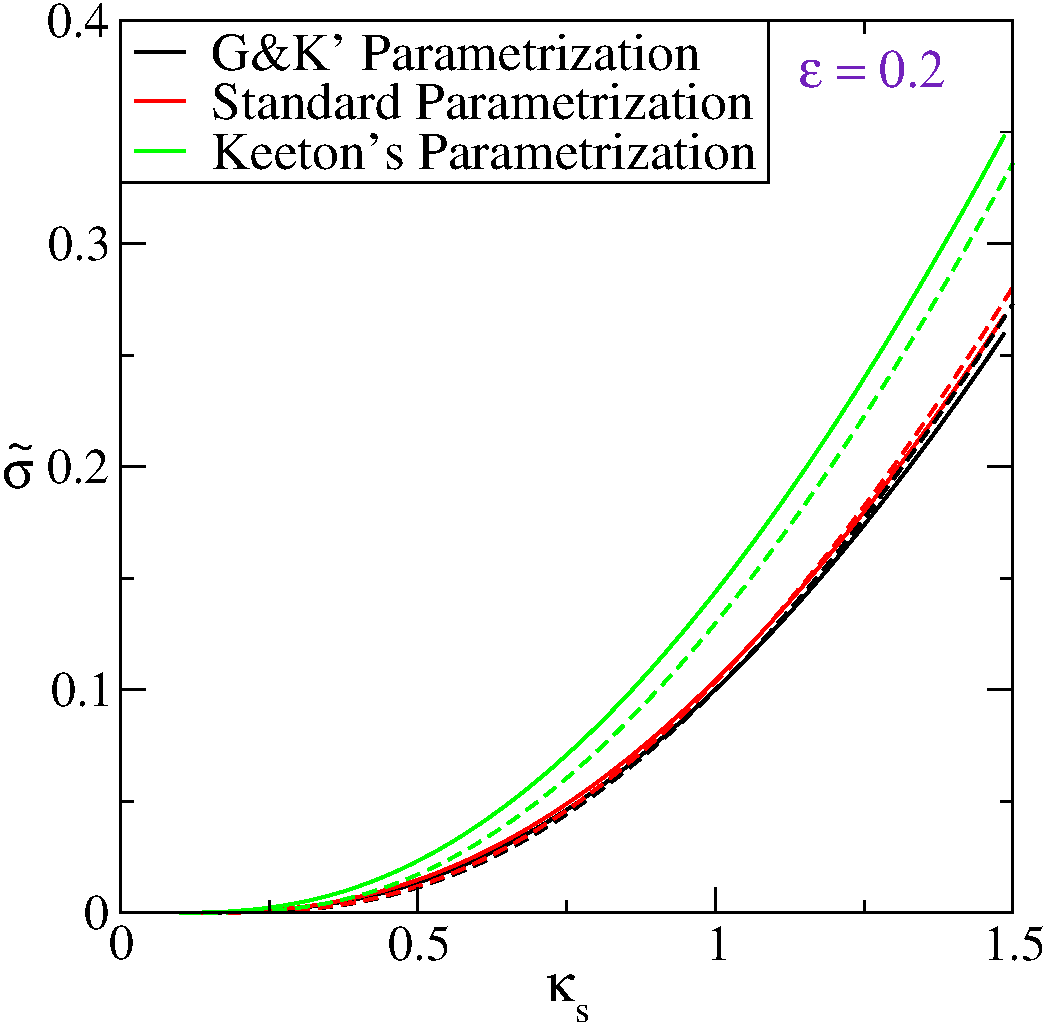
\includegraphics{graphics/dcs_ks_pnfw-pm.pdf}}
\hspace{3.cm}
\subfigure{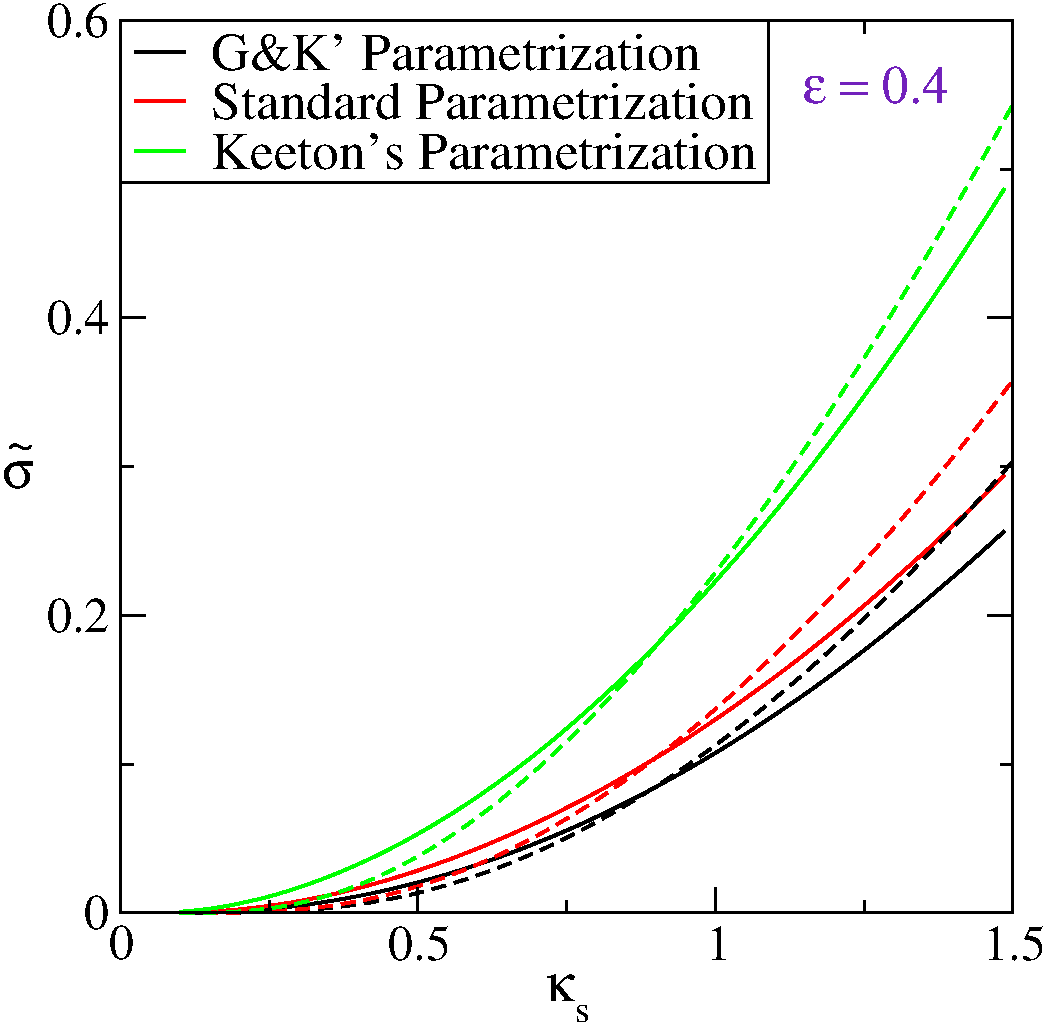
\includegraphics{graphics/dcs_ks_pnfw_e04-pm.pdf}}}
\caption{\label{siep_curves}  Cross Section for Deformation Arcs, calculated
for the PNFW model, as a function of $\kappa_s$ for two values of the parameter
$\varepsilon$. Solid-lines correspond to exact solution. Dashed-lines correspond
to Perturbative Approach. The calculations were done for $r_s=1$ and
$R_{\rm th}=10$.}
\end{figure*}


\begin{figure*}[!ht]
\resizebox{\hsize}{!}{
\subfigure{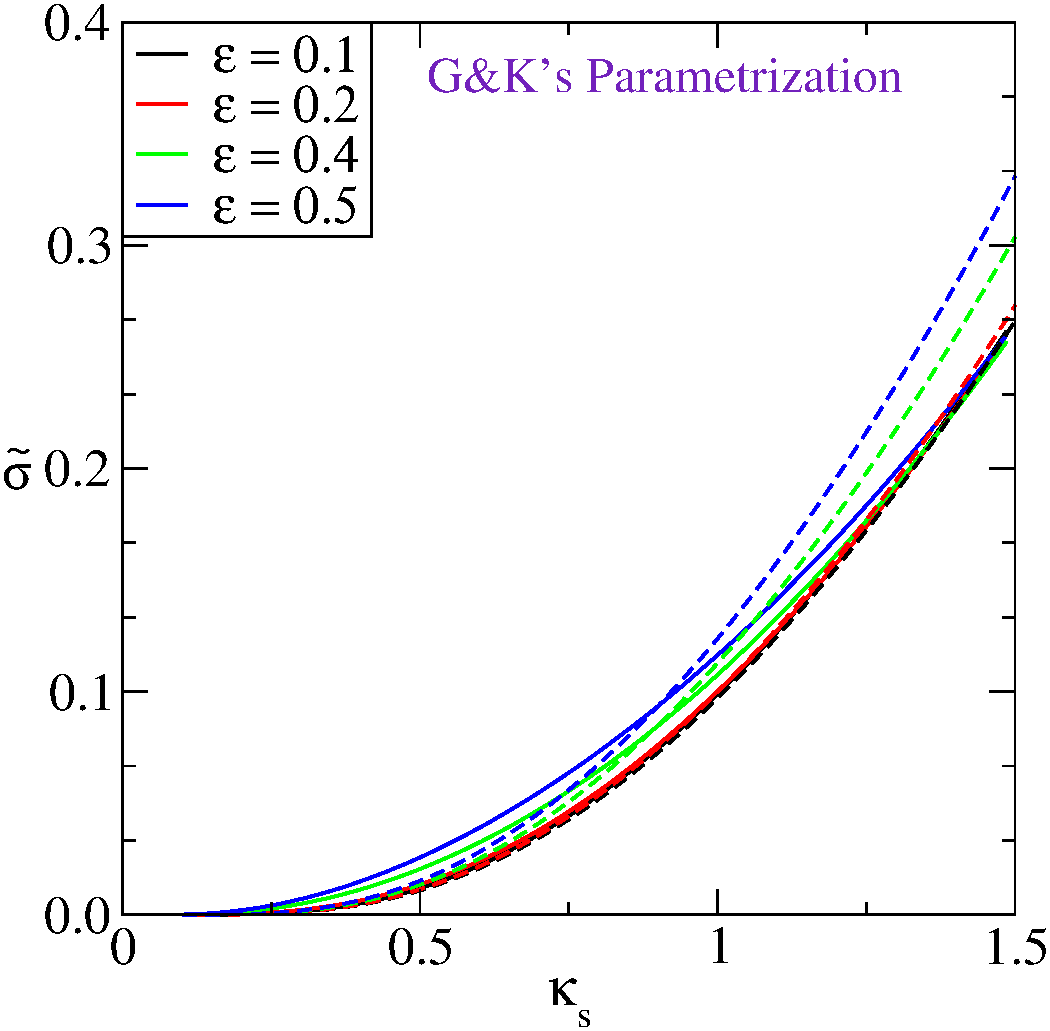
\includegraphics{graphics/dcs_pnfw_vs_ks-gk_pm.pdf}}\hspace{1.cm}
\subfigure{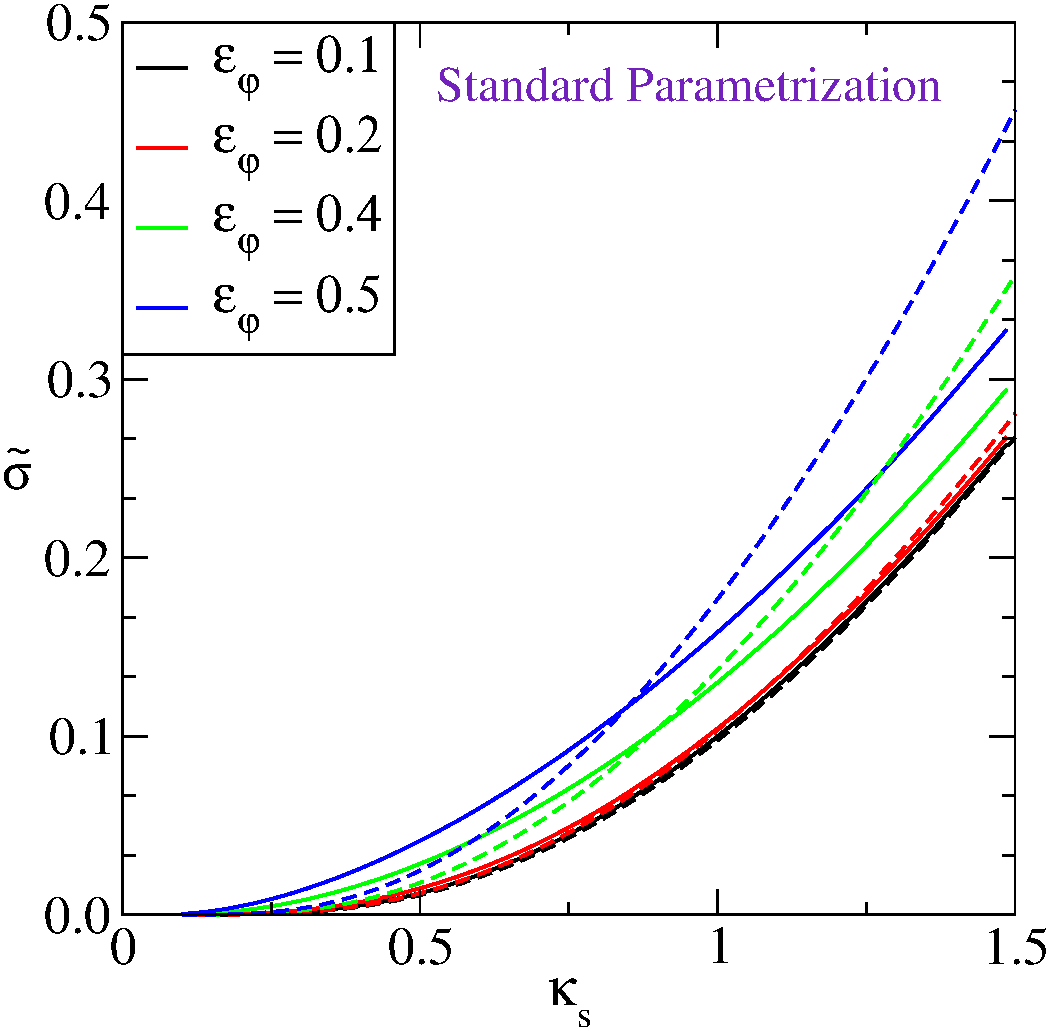
\includegraphics{graphics/dcs_pnfw_vs_ks-st_pm.pdf}}\hspace{1.cm}
\subfigure{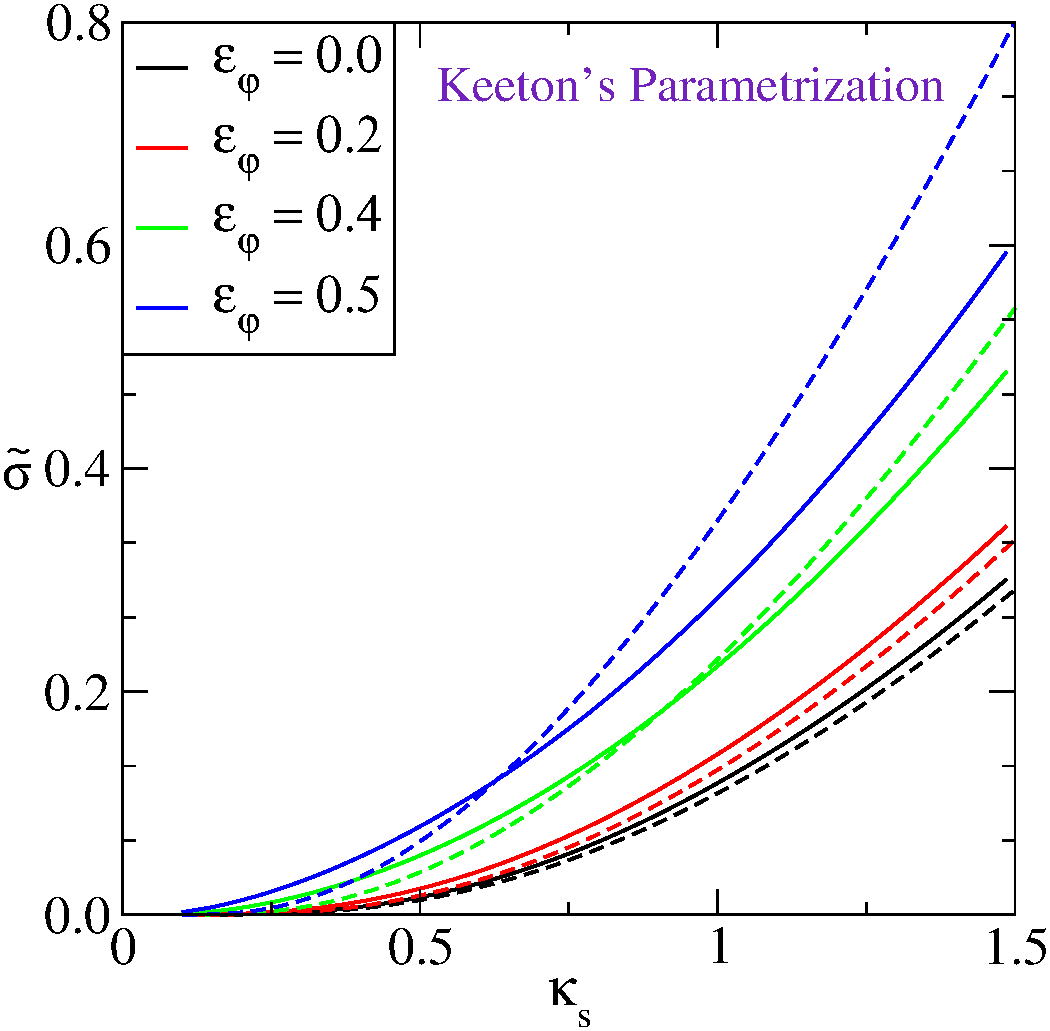
\includegraphics{graphics/dcs_pnfw_vs_ks-k_pm.pdf}}}
\caption{\label{dcs_pnfw_re_pm} Deformation cross section for the  PNFW lensing
model as a function of $\kappa_s$. Solid Lines correspond to the Exact
Solution. Dashed-Lines correspond to Perturbative Approach. Left Panel:
Parametrization of the Angle Deflection Model. Middle Panel: Standard
Parametrization. Right Panel: The Keeton's parametrization.  The calculations
were done for $R_{\rm th}=10$ and $r_s=1$.}
\end{figure*}

\begin{figure*}[!ht]
\resizebox{\hsize}{!}{
\subfigure{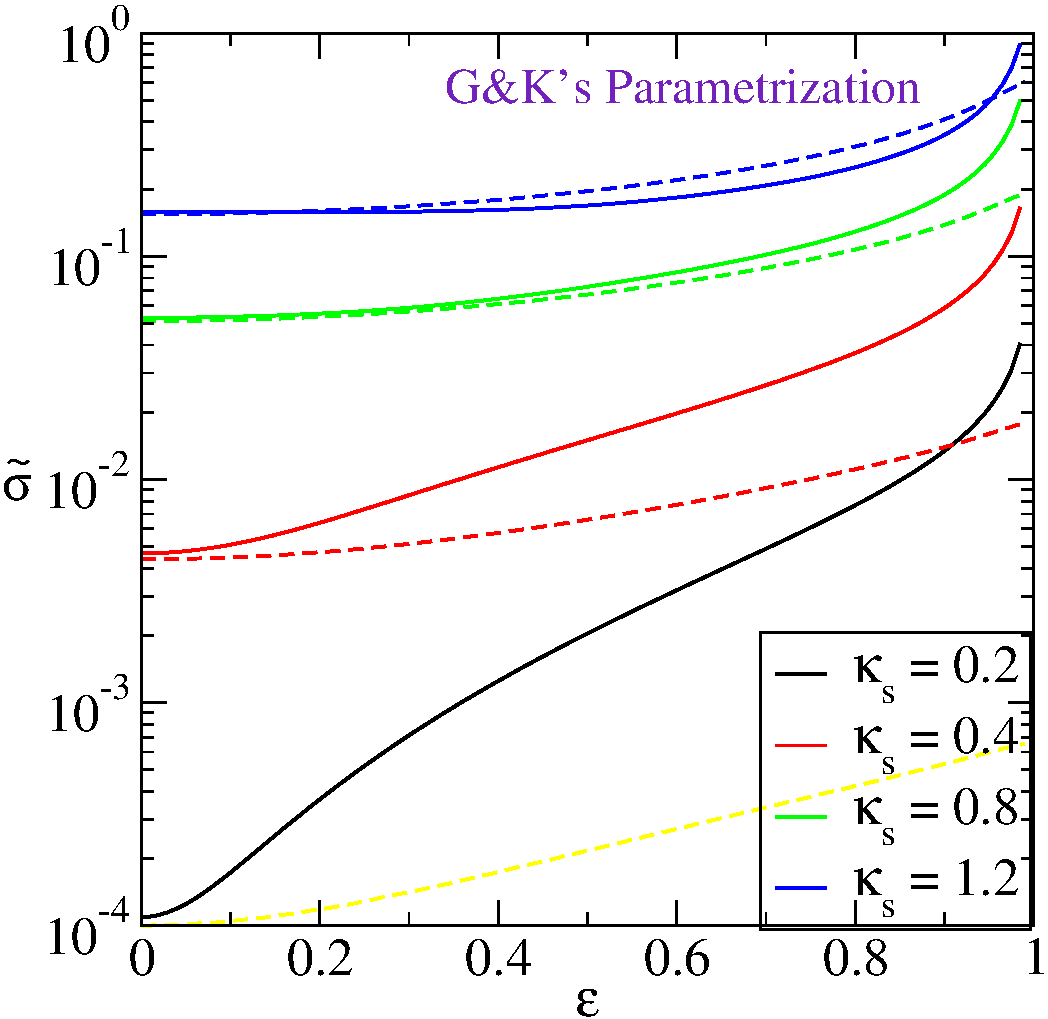
\includegraphics{graphics/dcs_pnfw_vs_e-gk_pm.pdf}}\hspace{1.cm}
\subfigure{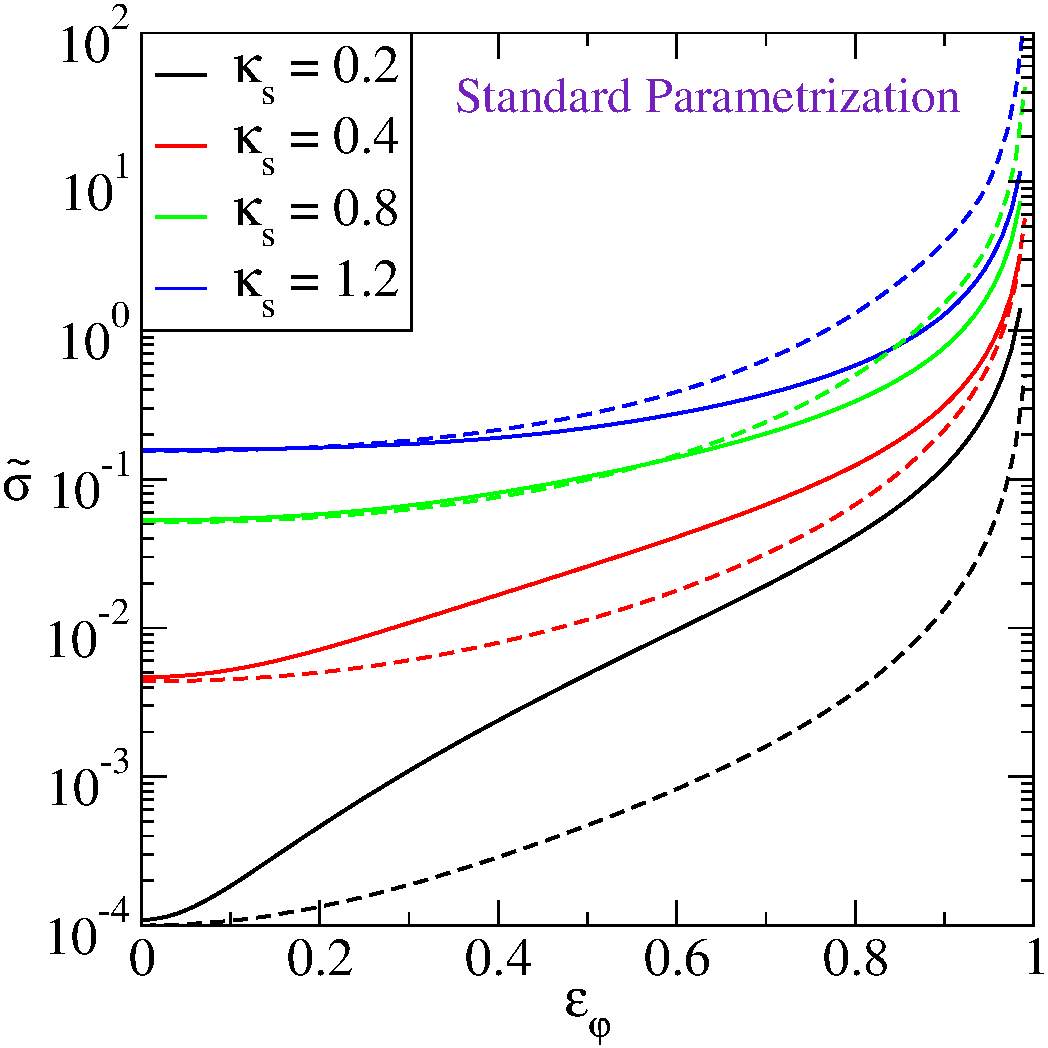
\includegraphics{graphics/dcs_pnfw_vs_e-st_pm.pdf}}\hspace{1.cm}
\subfigure{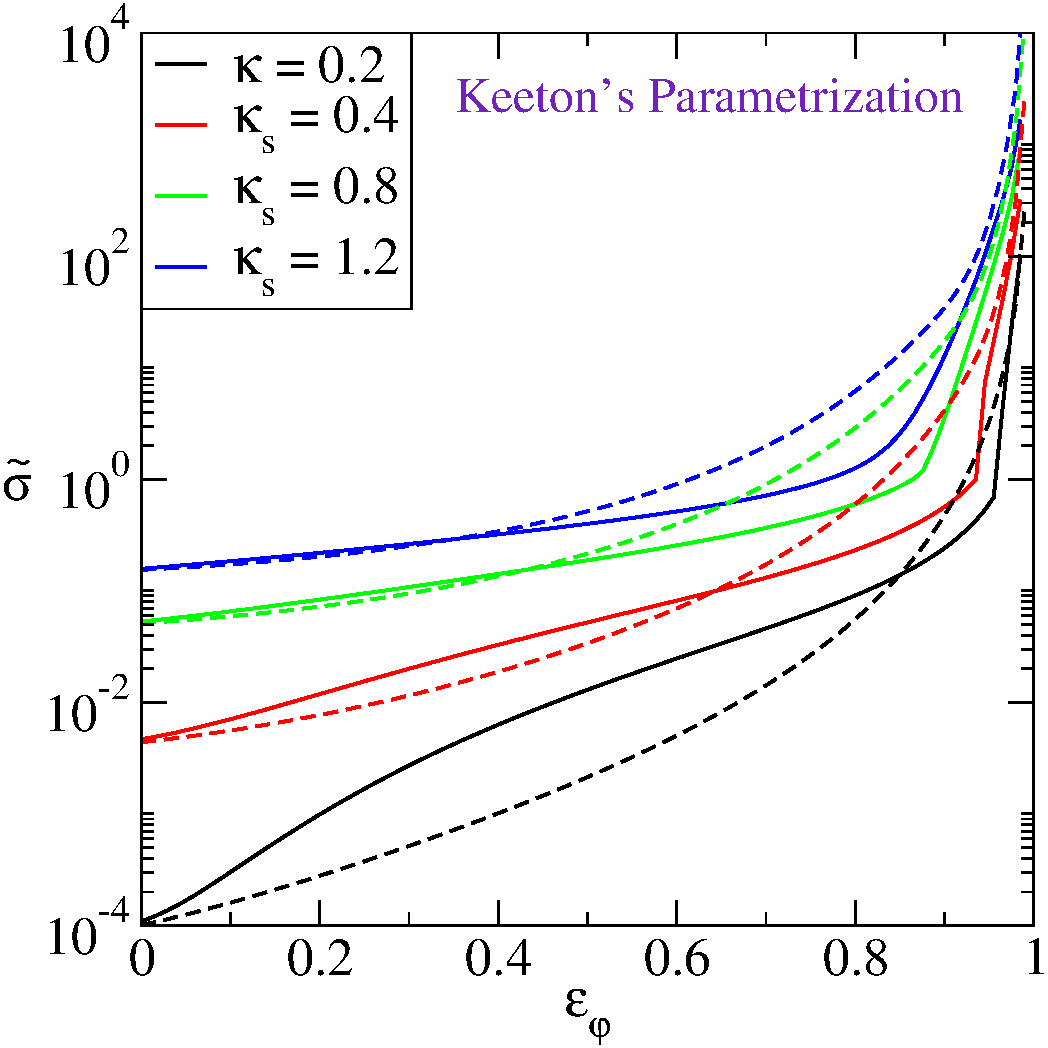
\includegraphics{graphics/dcs_pnfw_vs_e-k_pm.pdf}}}
\caption{\label{dcs_pnfw_e_pm} Deformation cross section for the  PNFW lensing
model as a function of the ellipticity. Solid Lines correspond to the Exact
Solution. Dashed-Lines correspond to Perturbative Approach. Left Panel:
Parametrization of the Angle Deflection Model. Middle Panel: Standard
Parametrization. Right Panel: The Keeton's parametrization. The calculations
were done for $R_{\rm th}=10$ and $r_s=1$.}
\end{figure*}

\begin{figure*}[!ht]
\resizebox{\hsize}{!}{
\subfigure{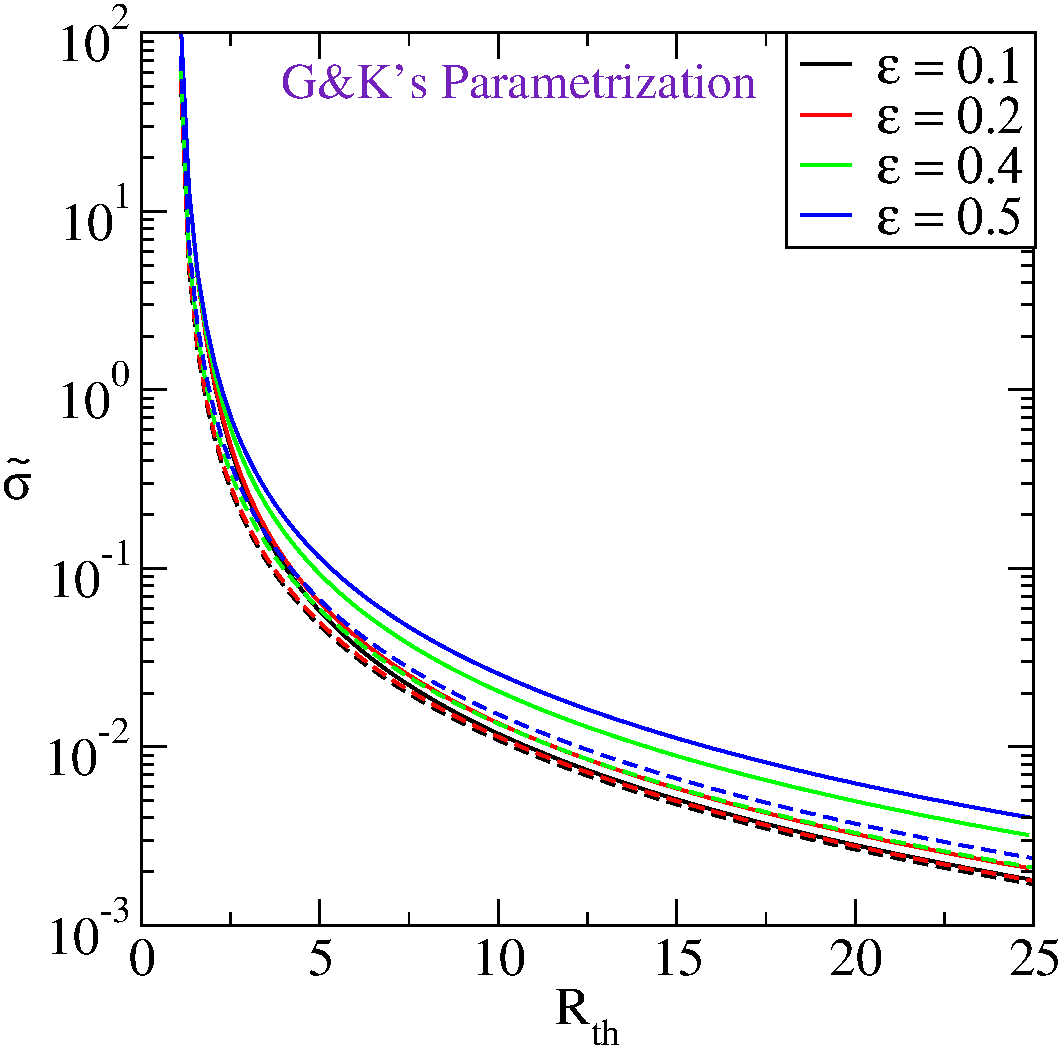
\includegraphics{graphics/dcs_pnfw_vs_rth-gk_pm.pdf}}\hspace{1.cm}
\subfigure{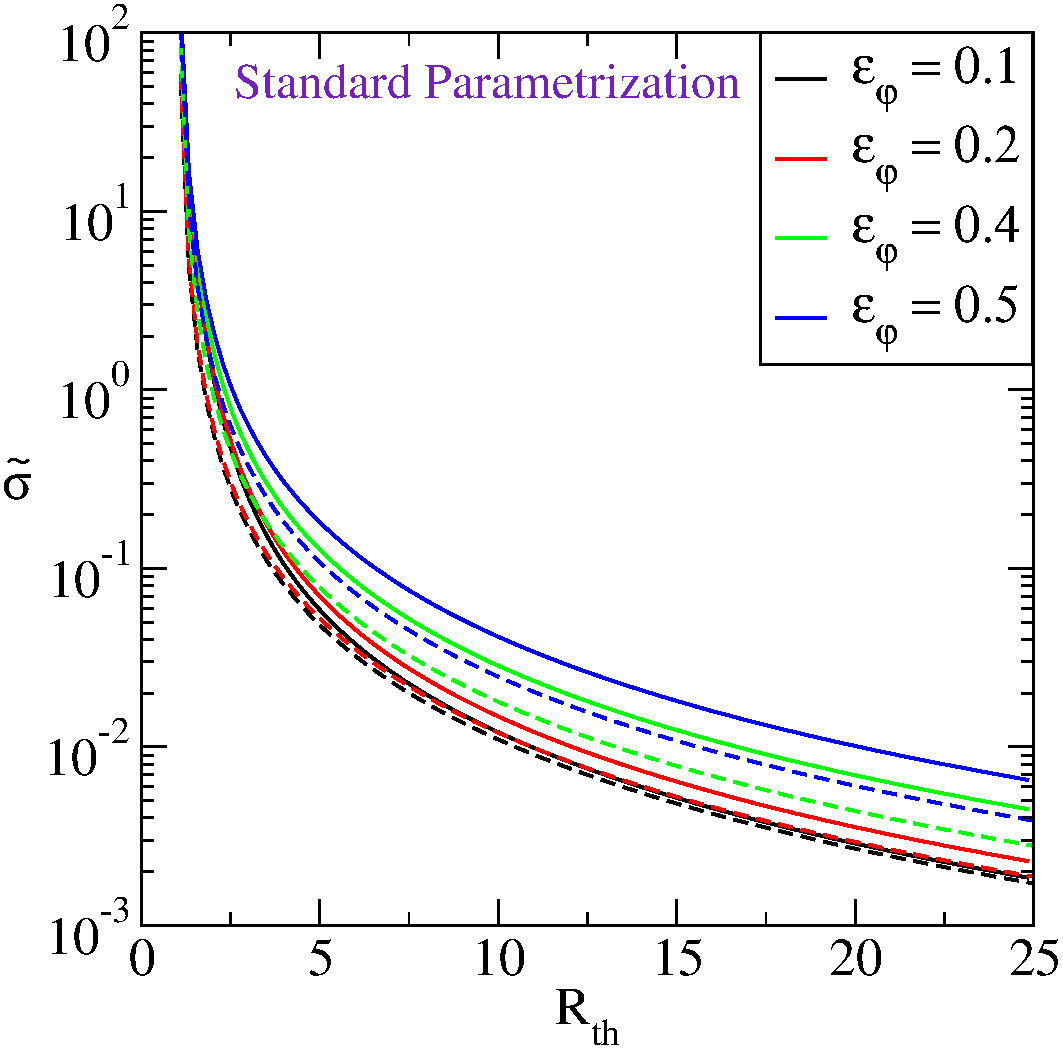
\includegraphics{graphics/dcs_pnfw_vs_rth-st_pm.pdf}}\hspace{1.cm}
\subfigure{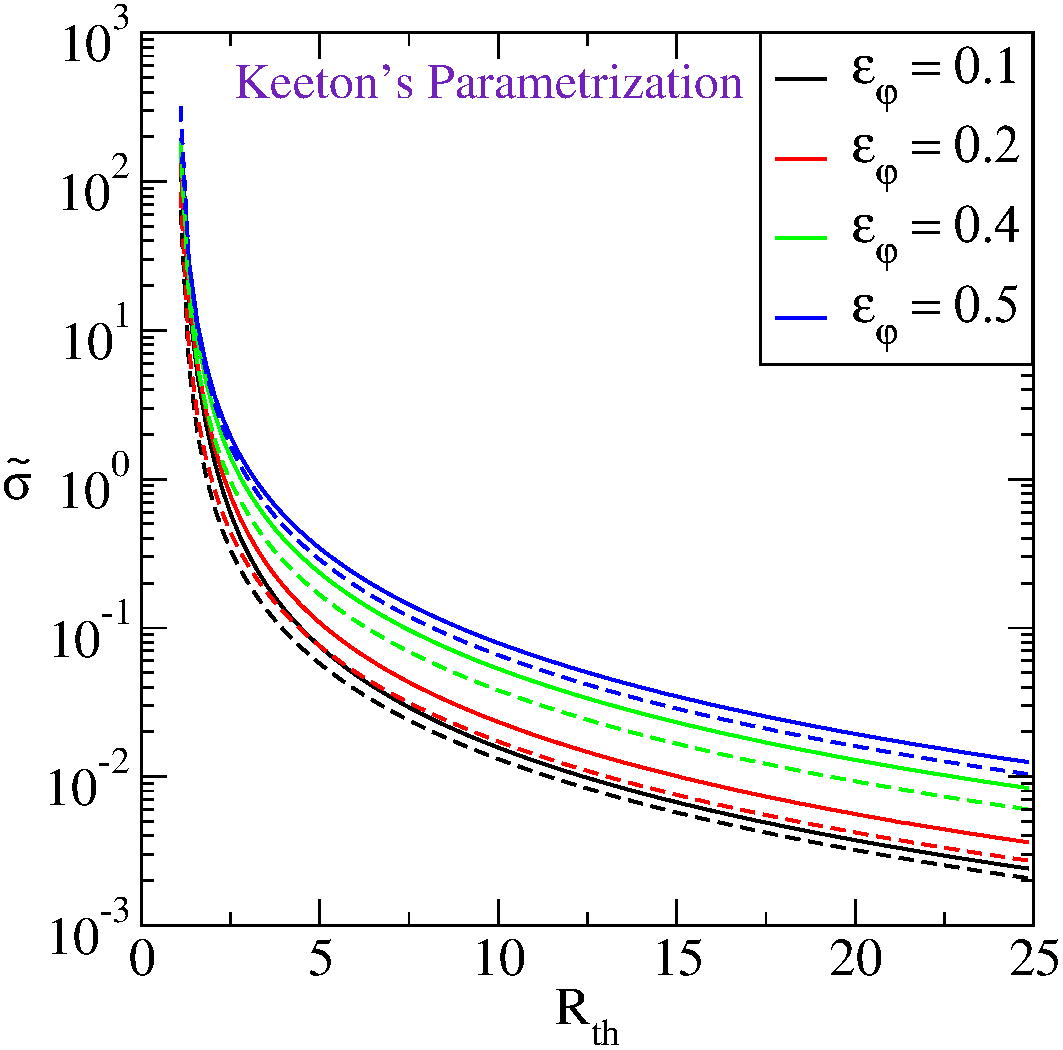
\includegraphics{graphics/dcs_pnfw_vs_rth-k_pm.pdf}}}
\caption{\label{dcs_pnfw_rth_pm} Deformation cross section for the  PNFW lensing
model as a function of $R_{\rm th}$. Solid Lines correspond to the Exact
Solution. Dashed-Lines correspond to Perturbative Approach. Left Panel:
Parametrization of the Angle Deflection Model. Middle Panel: Standard
Parametrization. Right Panel: The Keeton's parametrization. The calculations
were done for $\kappa_s=0.5$ and $r_s=1$.}
\end{figure*}

\chapter{Exact solution for Lens Models}

\section{Axially-Symmetric Models}

Include general description for this kind of models

\subsection{SIS}
The most single lens model for galaxies  corresponds to Singular Isothermal
Sphere. This model, is obtained by assuming a spherical mass distribution
that behaves as an isothermal gas in hidrostatic equilibrium. In this case,
the density is given by

\begin{equation}
 \rho(r)=\dfrac{\sigma_v^2}{2\pi G r^2},
\end{equation}
where $\sigma_v$ is the peculiar velocity  and $r=\sqrt{\xi^2+z^2}$ is the
distance to the center of the sphere. 

Choosing $\xi_0= \dfrac{4\pi \sigma^2_v D_{\rm LS} D_{\rm OS}}{c^2 D_{\rm
OS}}$ for the dimensionless coordinates $\vec{x}=\frac{\vec{\xi}}{\xi_0}$, the
lensing potential is given by

\begin{equation}
 \varphi(x)=x,
\label{sis_pot}
\end{equation}
where $x=\sqrt{x^2_1+x^2_2}$. From the lensing potential above, the lensing
functions are
\begin{eqnarray}
 \alpha(\vec{x}) &=& 1 \label{sis_angle}\\
\kappa(\vec{x}) &= & \dfrac{1}{2x} \label{sis_convg}\\
\gamma(\vec{x}) & = &  \dfrac{1}{2x} \label{sis_shear}.
\end{eqnarray}
Notice that, the vectorial expression for the deflection angle,
Eq.~(\ref{sis_angle}), is
\begin{equation}
 \vec{\alpha}(\vec{x})=\cos{\phi}\hat{\imath} + \sin{\phi}\hat{\jmath},
\end{equation}
where $\phi=\arctan{(x_2/x_1)}$.

For this model, the eigenvalues of the Jacobian matrix of lens mapping are:
\begin{eqnarray}
\lambda_r(x)&=&1 \label{lr_sis}\\
\lambda_t(x)&=&1-\dfrac{1}{x} \label{lt_sis}.
\end{eqnarray}

This is, the SIS model does not produce image elongated in the radial direction, therefore $x_{rcc}=0$ (the radial critical curve is degenerated into a point). The parametric equation of the radial caustic is
\begin{equation}
y_{1{\rm rca}}=-\cos{\phi}, \quad y_{2{\rm rca}}-\sin{\phi} \qquad \textrm{where\ } 0\leq \phi \leq 2\pi 
\end{equation}

However, the SIS produces images elongated in the tangential direction. The tangential critical curve is a circle of radius $x_{\rm tcc}=1$ (in dimension coordinates is a circle with radius $R_{\rm E}$). Then the parametric equation of the tangential critical curve is
\begin{equation}
x_{1{\rm tcc}}=x_{\rm tcc}\cos{\phi}, \quad x_{2{\rm tcc}}=x_{\rm tcc}\sin{\phi} \qquad \textrm{where\ } 0\leq \phi \leq 2\pi 
\end{equation}
And the tangential caustic is degenerated into a point, i.e.,
\begin{equation}
y_{1{\rm tca}}=0, \quad y_{2{\rm tcc}}=0 
\end{equation}

\subsection{NFW}

\section{Pseudo-Elliptical Models}
To distort a circular lensing potential $\varphi(x)$ into a elliptical shape $\varphi_\varepsilon(x)$, its radial
coordinate $x$ is replaced by $x_\varepsilon$, where $x_\varepsilon$ is given 
\begin{equation}
 x \rightarrow x_\varepsilon = \sqrt{x^2_{1\varepsilon}+x^2_{2\varepsilon}}=
\sqrt{a_{1\varepsilon}\,x^2_1+a_{2\varepsilon}\,x^2_2}.%
\label{subti-ellip}
\end{equation}

\noindent In general, for any choice of $a_{1\varepsilon}$ and
$a_{2\varepsilon}$, the lensing functions have simple analytical expressions.
For example, the angle deflection, convergence and the components of the
shear are 
\begin{eqnarray}
\vec{\alpha}_\varepsilon(\vec{x})&=&\alpha(x_\varepsilon)(\sqrt{a_{1\varepsilon}
} \cos { \phi_ \varepsilon},\sqrt{a_{2\varepsilon}}\sin{\phi_\varepsilon})
\label{ang_def_pe}\\
\kappa_\varepsilon(\vec{x})&=&\mathcal{A}(\varepsilon)\kappa(x_\varepsilon)
-\mathcal{B}(\varepsilon)\gamma(x_\varepsilon)\cos{2\phi_\varepsilon}
\label{kappa_pe}\\
\gamma_{1\varepsilon}(\vec{x})& = &
\mathcal{B}(\varepsilon)\kappa(x_\varepsilon)-\mathcal{A}
(\varepsilon)\gamma(x_\varepsilon)\cos{2\phi_\varepsilon} \\
\gamma_{2\varepsilon}(\vec{x})& =
&-\sqrt{\mathcal{A}^2(\varepsilon)-\mathcal{B}^2(\varepsilon)}
\gamma(x_\varepsilon)\sin{ 2\phi_\varepsilon}\\
\gamma^2_\varepsilon(\vec{x}) & = &
\mathcal{A}^2(\varepsilon)\gamma^2(x_\varepsilon)-2\mathcal{A}
(\varepsilon)\mathcal {B}
(\varepsilon)\kappa(x_\varepsilon)\gamma(x_\varepsilon)\cos{2\phi_\varepsilon}
\nonumber  \\ &  &
+\mathcal{B}^2(\varepsilon)[\kappa^2(x_\varepsilon)-\sin^2{2\phi_\varepsilon}
\gamma^2(x_\varepsilon) ]\label{gamma_pe}
\end{eqnarray}
\noindent where
$\phi_\varepsilon=\arctan(\frac{x_{2\varepsilon}}{x_{1\varepsilon}})$,
$\mathcal{A(\varepsilon)}=\frac{1}{2}(a_{1\varepsilon}+a_{2\varepsilon})$ and
$\mathcal{B}(\varepsilon)=\frac{1}{2}(a_{1\varepsilon}-a_{2\varepsilon})$.
$\kappa(x_\varepsilon)$
and $\gamma(x_\varepsilon)$ are respectively the convergence and shear of any
circular model, in
which $x$ was replaced by $x_\varepsilon$.


\subsection{SIEP}
For this kind of model, from Eq.~(\ref{sis_pot}) and Eq.~(\ref{subti-ellip})
the lensing potential reads
\begin{equation}
 \varphi_\varepsilon(\vec{x})=x_\varepsilon,\label{siep_pot}
\end{equation}
 and its lensing functions are
\begin{eqnarray}
\vec{\alpha}_\varepsilon(\vec{x}) & = & (\sqrt{a_{1\varepsilon}
} \cos { \phi_ \varepsilon},\sqrt{a_{2\varepsilon}}\sin{\phi_\varepsilon})\\
\kappa_\varepsilon(\vec{x}) & = &
\left[\mathcal{A}(\varepsilon)-\mathcal{B}(\varepsilon)\cos{2\phi_\varepsilon}
\right](2 x_\varepsilon)^{-1}=\gamma_\varepsilon(\vec{x})
\end{eqnarray}
From the equations above, the components of the lens equation are
\begin{eqnarray}
 y_1&=&\dfrac{x_\varepsilon\cos{\phi_\varepsilon}}{\sqrt{a_{1\varepsilon}}}-\sqrt{a_{1\varepsilon}}\cos{\phi_ \varepsilon} \label{y1_siep}\\
y_2&=&\dfrac{x_\varepsilon\sin{\phi_\varepsilon}}{\sqrt{a_{2\varepsilon}}}-\sqrt{a_{2\varepsilon}}\sin{\phi_ \varepsilon} \label{y2_siep},
\end{eqnarray}
and the expression for the eigenvalues read
\begin{eqnarray}
\lambda_r(\vec{x})&=& 1-\kappa_\varepsilon(\vec{x})+\gamma_\varepsilon(\vec{x} )=1 \label{lr_siep}\\
\lambda_t(\vec{x})& =& 1-\kappa_\varepsilon(\vec{x})-\gamma_\varepsilon(\vec{x}
)=1-\left[\mathcal{A}(\varepsilon)-\mathcal{B}(\varepsilon)\cos{2\phi_\varepsilon } \right](x_\varepsilon)^{-1} \label{lt_siep}
\end{eqnarray}

From the Eq.~(\ref{lr_siep}) since $\lambda_r=1$ is not null, the radial critical curve is degenerated into a point $x_{rcc}=0$, and therefore the components of the radial caustic is
 \begin{eqnarray}
y_{1,rca} &=&-\sqrt{a_{1\varepsilon}}\cos{\phi_ \varepsilon}\\
y_{2,rca} &=&-\sqrt{a_{2\varepsilon}}\sin{\phi_ \varepsilon},
\end{eqnarray}

From the Eq.~(\ref{lt_siep}) the pseudo-elliptical radial coordinate of the tangential critical curve  ($\lambda_t=0$) is
\begin{equation}
x_{\varepsilon,tcc}= \mathcal{A}(\varepsilon)-\mathcal{B}(\varepsilon)\cos{2\phi_\varepsilon}, 
\end{equation}
then, the cartesian coordinates of the tangential critical are
\begin{equation}
x_{1,tcc}=\dfrac{x_{\varepsilon,tcc}\cos{\phi_\varepsilon}}{\sqrt{a_{1\varepsilon}}},\qquad x_{2,tcc}=\dfrac{x_{\varepsilon,tcc}\sin{\phi_\varepsilon}}{\sqrt{a_{2\varepsilon}}},
\end{equation}
and the componente of the tangential caustic are
\begin{eqnarray}
y_{1,tca} &=&x_{1,tcc}-\sqrt{a_{1\varepsilon}}\cos{\phi_\varepsilon}\\
y_{2,tca} &=&x_{2,tcc}-\sqrt{a_{2\varepsilon}}\sin{\phi_\varepsilon},
\end{eqnarray}

Besides, the local approximation for the length-to-width ratio of arcs $R_\lambda:=\lambda_r/\lambda_t$ implies
\begin{equation}
R_{\rm th}=\dfrac{1}{1-\left[\mathcal{A}(\varepsilon)-\mathcal{B}(\varepsilon)\cos{2\phi_\varepsilon } \right](x_\varepsilon)^{-1}},
\end{equation}
and the pseudo-elliptical radial coordinates of the curves of constant distortion (in the lens plane) are
\begin{equation}
x_{\varepsilon,R_{\rm th}}=x_{\varepsilon,tcc}\times\left\{\begin{array}{cc} \dfrac{|R_{\rm th}|}{|R_{\rm th}|-1}, & R_{\rm th}>0 \\ & \\
\dfrac{|R_{\rm th}|}{|R_{\rm th}|+1}, & R_{\rm th}<0 \end{array}\right.
\end{equation}
The cartesian components of the cuves of constant distortion in the source plane are given by the Eqs.~(\ref{y1_siep}) and (\ref{y2_siep}) where $x_\varepsilon$ is replaced by $x_{\varepsilon,R_{\rm th}}$.

In Fig.~\ref{siep_curves} we show an example for the main curves of the SIEP model in both planes, for $R_{\rm E}=1$, $\varepsilon=0.4$ (that corresponds to the lensing potential ellipticity by itself).

\begin{figure*}[!ht]
\resizebox{\hsize}{!}{
\subfigure{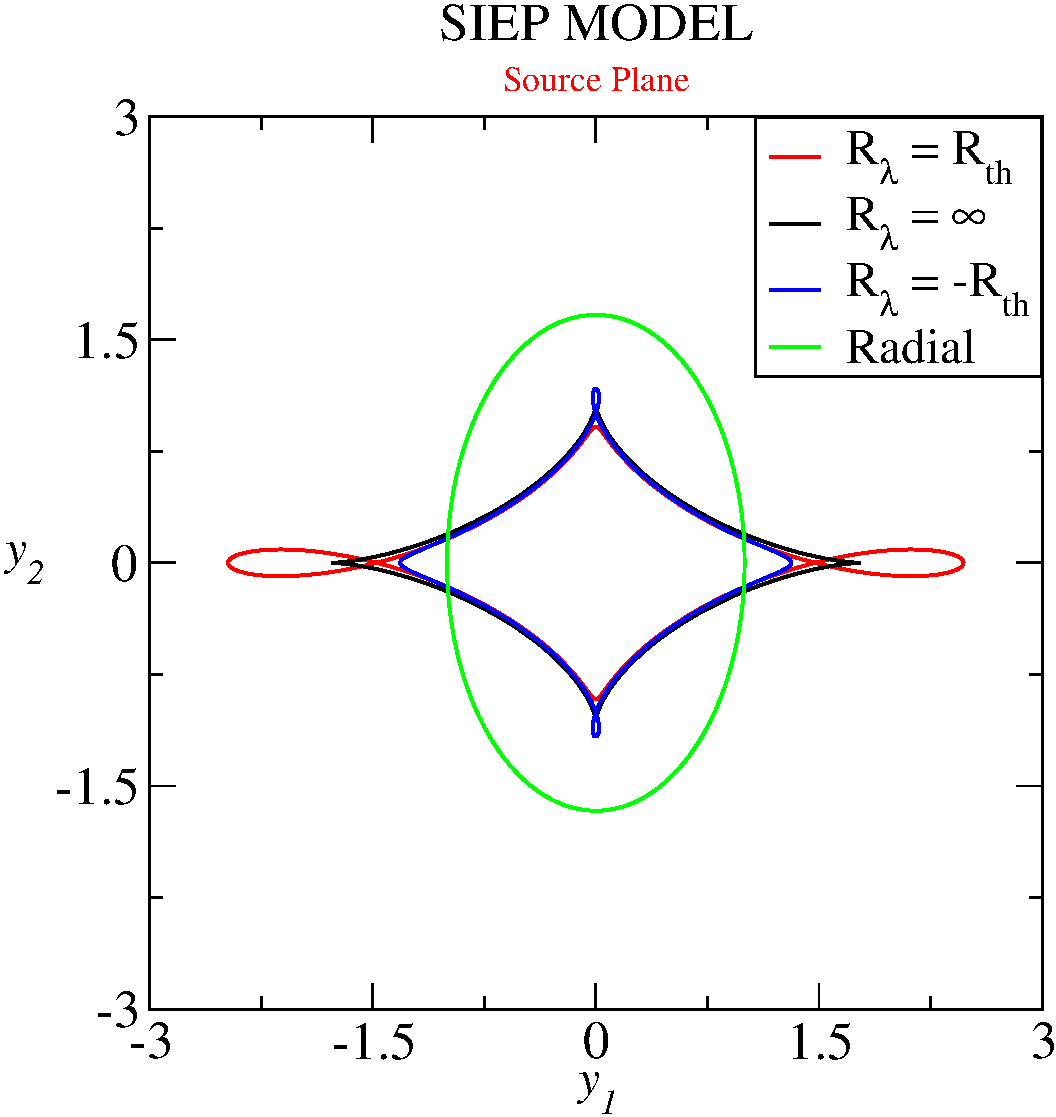
\includegraphics{graphics/siep_source_plane.pdf}}
\hspace{3.cm}
\subfigure{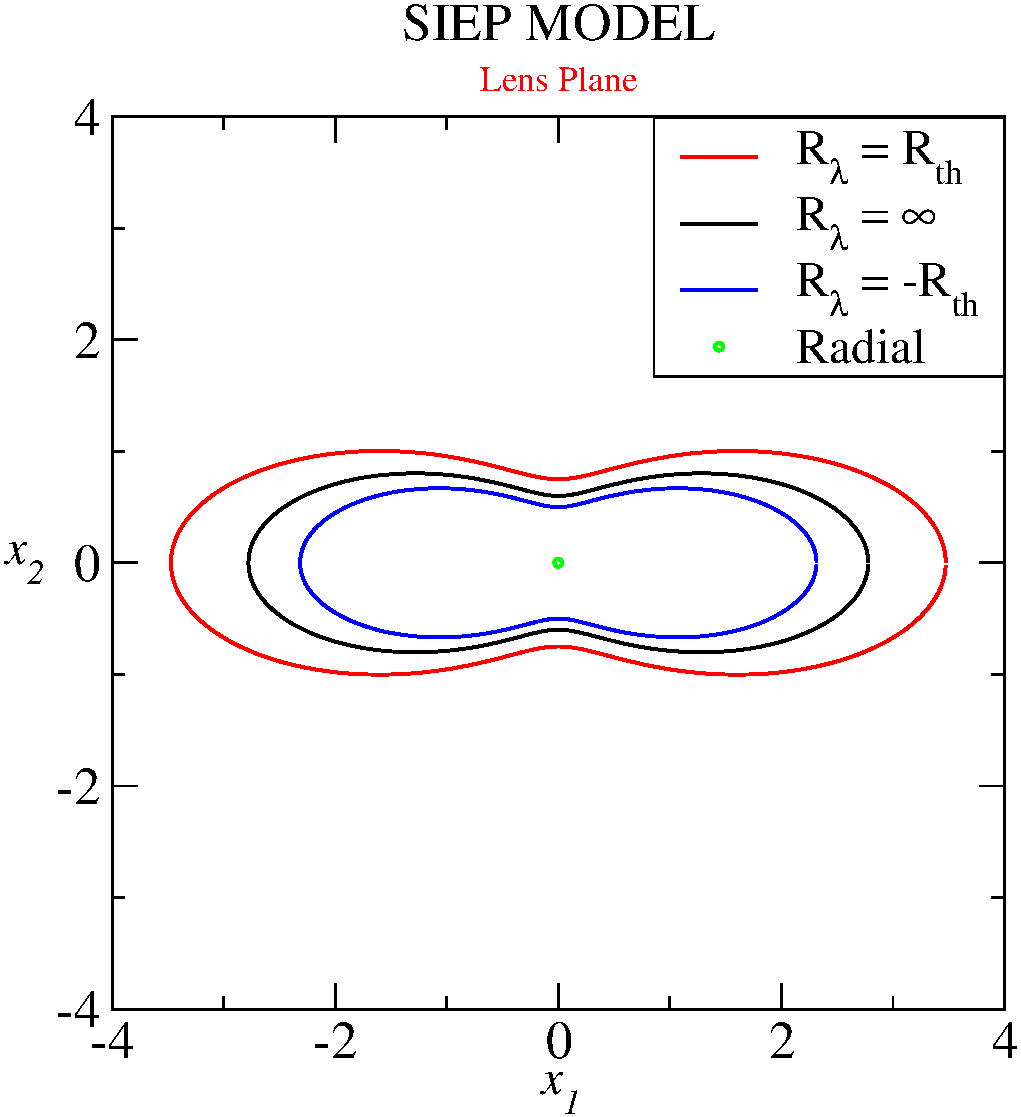
\includegraphics{graphics/siep_lens_plane.pdf}}}
\caption{\label{siep_curves}  SIEP lensing model curves. Left Panel:
Tangential($R_\lambda=\infty$) and Radial Caustics and Curves of Constant
Distortion ($R_\lambda=\pm R_{\rm th}$) . Right Panel: Tangential
($R_\lambda=\infty$) and Radial Critical Curves and  Constant Distortion Curves
($R_\lambda=\pm R_{\rm th}$). Here, we used $R_{\rm E}=1$ and $|R_{\rm
th}|=5$ and the Keeton's parametrization,i.e,  $a_{1\varepsilon}=1$ and
$a_{2\varepsilon}=(1-\varepsilon)^{-2}$ for $\varepsilon=0.4$, }
\end{figure*}


\section{Elliptical Models}

\section{Arc Cross Section}
In this work, we compute the Arc Cross Section by using the local approximation for the length-to-width ratio of arcs, we substitute $L/W$ by 
\begin{equation}
R_\lambda:=\dfrac{\lambda_r}{\lambda_t},
\end{equation}
and the condition for minimum distortion is given by a number $R_{\rm th}$.  When we use this local measurement for the properties of the arcs, we are considering only deformation arcs and therefore, we are calculating the cross section for deformation arcs $\sigma_{\rm dcs}$

\begin{equation}
\sigma_{\rm dcs} \equiv \int d^2\eta =\int_{ \frac{\lambda_r}{\lambda_t} > |R_{\rm th}|} \left |{\rm det}\,\textbf{J}(\vec{\xi}) \right| d^2\xi.
\end{equation}

However, as we are working with dimensionless coordinates $ \vec{y}=\frac{\eta}{\eta_0}$ and $\vec{x}=\frac{\xi}{\xi_0}$ we can write $\sigma_{\rm dcs}$ as
\begin{equation}
\sigma_{\rm dcs} = \xi_0^2\tilde{\sigma}_{\rm dcs}= \xi_0^2 \int_{ \frac{\lambda_r}{\lambda_t} > |R_{\rm th}|} \left |{\rm det}\,\textbf{J}(\vec{x}) \right| d^2\!x. \label{dcs_dimensionless}
\end{equation}

In general, the calculation of theses expression requires numerical method, unless for a few kind of lens model.  For example, for the SIS model, $\mathbf{J}(\vec{x})=1-\frac{1}{x}$, $\xi_0=\re$ and, hence we have

\begin{equation}
\sigma_{dcs}=2\pi\,R^2_{\rm E} \dfrac{|R_{\rm th}|^2+1}{(|R_{\rm th}|^2-1)^2} \label{dcs_sis}
\end{equation}

Note that the last equation is the same as the Eq.~(\ref{dcs_sis_pertapp}). The other model that offers an analytical expression for the cross section for deformation arcs is the SIEP. For this model, first we have that the determinant of the Jacobian matrix is
\begin{equation}
\mathbf{J}(\vec{x})=1-\dfrac{x_{\varepsilon,tcc}}{x_{\varepsilon}}, \label{jacob_siep}
\end{equation}
where $x_{\varepsilon,tcc}$ corresponds to the radial coordinate of the tangential critical curve. Then, by inserting the last equation in Eq.~(\ref{dcs_dimensionless}), and $d^2\,x=xdx d\phi$, we have

\begin{equation}
\tilde{\sigma}_{\rm siep}= \int_{0}^{2\pi}\int_{x_{_{-R_{\rm th}}}}^{x_{_{R_{\rm th}}}}\left| 1-\dfrac{x_{\varepsilon,tcc}}{x_{\varepsilon}}\right| x dx d\phi 
\end{equation}
As in polar coordinates $x_{\varepsilon}=xf(\phi)$, where $f(\phi)=\sqrt{a_{1\varepsilon}\cos^2{\phi}+a_{2\varepsilon}\sin^2{\phi}}$, the result integration in the radial coordinate is
\begin{equation}
\tilde{\sigma}_{\rm siep}= \dfrac{|R_{\rm th}|^2+1}{(|R_{\rm th}|^2-1)^2} \int_{0}^{2\pi}\left[\mathcal{A}(\varepsilon)-\mathcal{B}(\varepsilon)\cos{(2\phi_\varepsilon)} \right] d\phi 
\end{equation}
Therefore, the analytical expression for the deformation cross section for the SIEP is
 \begin{equation}
\sigma_{\rm siep}= R^2_{\rm E}\dfrac{|R_{\rm th}|^2+1}{(|R_{\rm th}|^2-1)^2} \left[2\pi\left[\mathcal{A}(\varepsilon)+\mathcal{B}(\varepsilon)\right]-2\sqrt{\dfrac{a_{1\varepsilon}}{a_{2\varepsilon}}}\mathcal{B}(\varepsilon)\arctan{\left(2\pi\sqrt{\dfrac{a_{2\varepsilon}}{a_{1\varepsilon}}}\right)} \right]
\end{equation}
In the limit $\varepsilon \rightarrow 0$, we have that $\mathcal{A}(\varepsilon)=1$, $\mathcal{B}(\varepsilon)=0$, and the expression above is the same as Eq.~(\ref{dcs_sis})

\begin{figure*}[!ht]
\resizebox{\hsize}{!}{
\subfigure{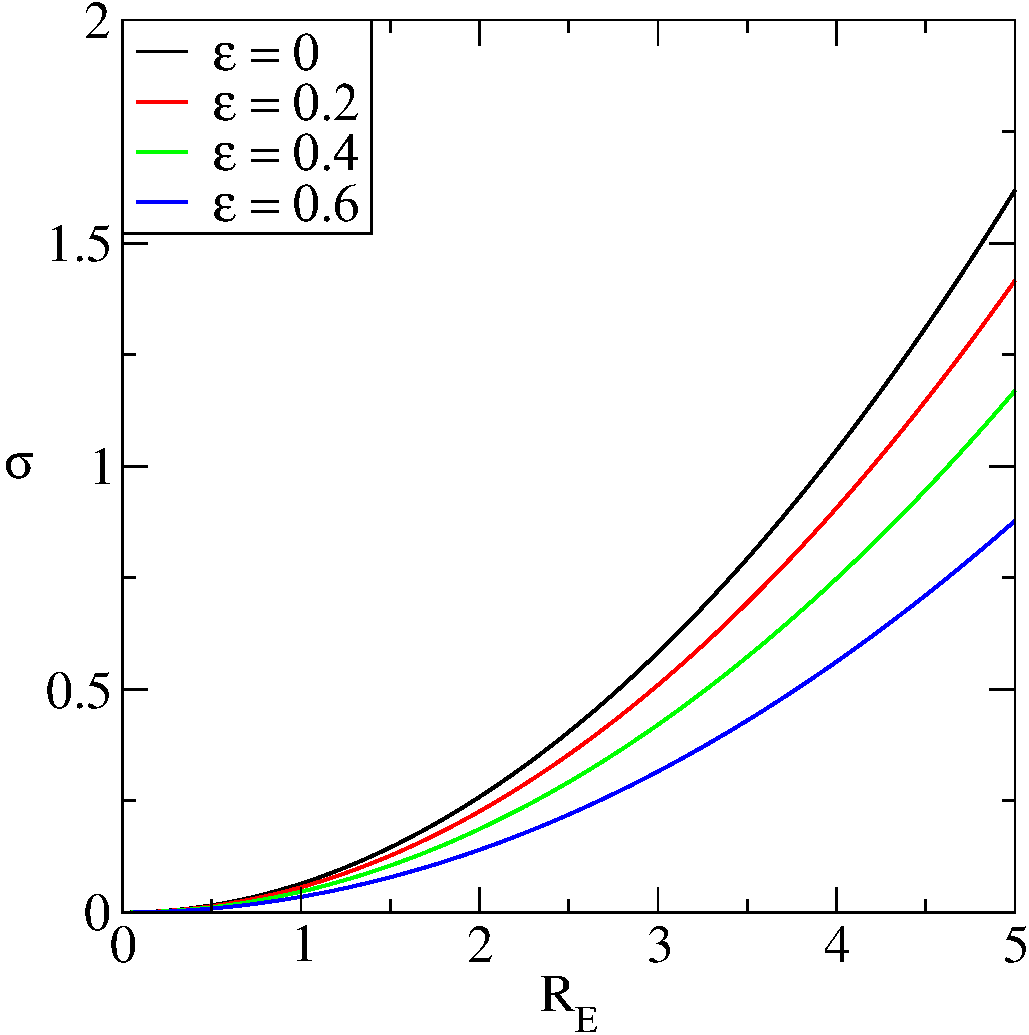
\includegraphics{graphics/dcs_siep_vs_re.pdf}}
\hspace{3.cm}
\subfigure{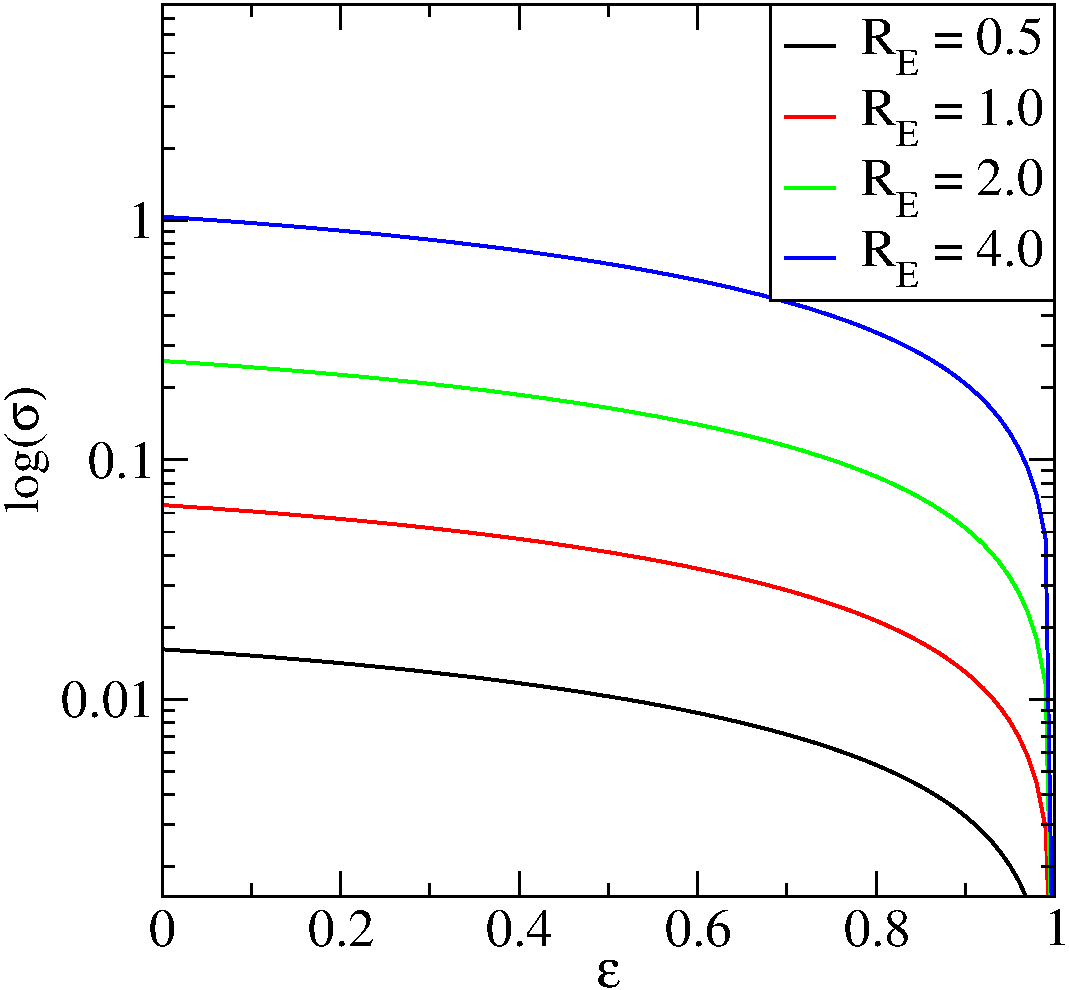
\includegraphics{graphics/dcs_siep_vs_e.pdf}}}
\caption{\label{dcs_siep} Deformation cross section for the  SIEP lensing model. Left Panel:
$\sigma$ as a function of $R_{\rm E}$. Right Panel: $\sigma$ as a function of $\varepsilon$.
The calculation were made for $R_{\rm th}=10$.
}
\end{figure*}

\addcontentsline{toc}{chapter}{References}

% Rough biblio, i'm sure it needs format changes, but it's a start
% Started Dec 6, 2010 by MSSG

\begin{thebibliography}{99}

\bibitem[\protect{Ferreira, P.}(2010)]{pedrothesis} Ferreira, P., Master's Thesis
\bibitem[\protect{De Bom, C.}(2010)]{clecio} De Bom, C. method for measuring arc length.

\bibitem[\protect{Golse \& Kneib}(2002)]{golsekneib} Golse \& Kneib

\bibitem[\protect{Meneghetti et al}(2002)]{meneg} Meneghetti et al

% \bibitem[\protect{

\end{thebibliography}



%\input{bibliografia}
%\input{biblio-modi}
\end{document}

% \begin{center}
% \fboxrule6pt
% \fcolorbox
% {red!70!green}% outer frame
% {yellow!30!blue}% outer background
% {\fcolorbox
% {-yellow!30!blue}% inner frame
% {-red!70!green}% inner background
% {\begin{minipage}{10cm}
% {\it
% texto
% }
%  \end{minipage}
% }}
% \end{center}
